\documentclass{article}
\usepackage[final]{neurips_2025}  % NEURIPS style (neurips_2025.sty is in paper_draft/)
% [final] alone sets no track; provide the main-track footer text
\makeatletter\providecommand{\@trackname}{\@neuripsordinal\ Conference on Neural Information Processing Systems (NeurIPS \@neuripsyear).}\makeatother
\usepackage[hidelinks]{hyperref}  % REQUIRED: clickable links
\usepackage{booktabs}  % REQUIRED: professional tables
\usepackage{graphicx}
\usepackage{amsmath,amssymb}
\usepackage[utf8]{inputenc}
\usepackage[T1]{fontenc}
\usepackage{subcaption}
\usepackage{enumitem}
\usepackage{multirow}
\usepackage{algorithm}
\usepackage[noend]{algpseudocode}

% Import command files
%%%%% MATH NOTATION MACROS %%%%%
% Standard math notation for academic papers
% Import with: %%%%% MATH NOTATION MACROS %%%%%
% Standard math notation for academic papers
% Import with: %%%%% MATH NOTATION MACROS %%%%%
% Standard math notation for academic papers
% Import with: \input{commands/math}

\usepackage{amsmath,amsfonts,bm}

%%%%%%%%%%%%%%%%%%%%%%%%%%%%%%%%%%%%%%%%%%%%%%%%%%%%%%%%%%%%%%%%%
% FIGURE AND SECTION REFERENCES
%%%%%%%%%%%%%%%%%%%%%%%%%%%%%%%%%%%%%%%%%%%%%%%%%%%%%%%%%%%%%%%%%

% Mark sections of captions for referring to divisions of figures
\newcommand{\figleft}{{\em (Left)}}
\newcommand{\figcenter}{{\em (Center)}}
\newcommand{\figright}{{\em (Right)}}
\newcommand{\figtop}{{\em (Top)}}
\newcommand{\figbottom}{{\em (Bottom)}}
\newcommand{\captiona}{{\em (a)}}
\newcommand{\captionb}{{\em (b)}}
\newcommand{\captionc}{{\em (c)}}
\newcommand{\captiond}{{\em (d)}}

% Figure references
\def\figref#1{figure~\ref{#1}}
\def\Figref#1{Figure~\ref{#1}}
\def\twofigref#1#2{figures \ref{#1} and \ref{#2}}
\def\quadfigref#1#2#3#4{figures \ref{#1}, \ref{#2}, \ref{#3} and \ref{#4}}

% Section references
\def\secref#1{section~\ref{#1}}
\def\Secref#1{Section~\ref{#1}}
\def\twosecrefs#1#2{sections \ref{#1} and \ref{#2}}
\def\secrefs#1#2#3{sections \ref{#1}, \ref{#2} and \ref{#3}}

% Equation references
\def\eqref#1{equation~\ref{#1}}
\def\Eqref#1{Equation~\ref{#1}}
\def\plaineqref#1{\ref{#1}}

% Algorithm references
\def\algref#1{algorithm~\ref{#1}}
\def\Algref#1{Algorithm~\ref{#1}}
\def\twoalgref#1#2{algorithms \ref{#1} and \ref{#2}}
\def\Twoalgref#1#2{Algorithms \ref{#1} and \ref{#2}}

% Table references
\def\tabref#1{table~\ref{#1}}
\def\Tabref#1{Table~\ref{#1}}

% Chapter references
\def\chapref#1{chapter~\ref{#1}}
\def\Chapref#1{Chapter~\ref{#1}}

%%%%%%%%%%%%%%%%%%%%%%%%%%%%%%%%%%%%%%%%%%%%%%%%%%%%%%%%%%%%%%%%%
% BASIC MATH DEFINITIONS
%%%%%%%%%%%%%%%%%%%%%%%%%%%%%%%%%%%%%%%%%%%%%%%%%%%%%%%%%%%%%%%%%

\def\ceil#1{\lceil #1 \rceil}
\def\floor#1{\lfloor #1 \rfloor}
\def\1{\bm{1}}
\def\eps{{\epsilon}}

% Common operators
\DeclareMathOperator*{\argmax}{arg\,max}
\DeclareMathOperator*{\argmin}{arg\,min}
\DeclareMathOperator{\sign}{sign}
\DeclareMathOperator{\Tr}{Tr}
\let\ab\allowbreak

%%%%%%%%%%%%%%%%%%%%%%%%%%%%%%%%%%%%%%%%%%%%%%%%%%%%%%%%%%%%%%%%%
% VECTORS (lowercase bold)
%%%%%%%%%%%%%%%%%%%%%%%%%%%%%%%%%%%%%%%%%%%%%%%%%%%%%%%%%%%%%%%%%

\def\vzero{{\bm{0}}}
\def\vone{{\bm{1}}}
\def\vmu{{\bm{\mu}}}
\def\vtheta{{\bm{\theta}}}
\def\va{{\bm{a}}}
\def\vb{{\bm{b}}}
\def\vc{{\bm{c}}}
\def\vd{{\bm{d}}}
\def\ve{{\bm{e}}}
\def\vf{{\bm{f}}}
\def\vg{{\bm{g}}}
\def\vh{{\bm{h}}}
\def\vi{{\bm{i}}}
\def\vj{{\bm{j}}}
\def\vk{{\bm{k}}}
\def\vl{{\bm{l}}}
\def\vm{{\bm{m}}}
\def\vn{{\bm{n}}}
\def\vo{{\bm{o}}}
\def\vp{{\bm{p}}}
\def\vq{{\bm{q}}}
\def\vr{{\bm{r}}}
\def\vs{{\bm{s}}}
\def\vt{{\bm{t}}}
\def\vu{{\bm{u}}}
\def\vv{{\bm{v}}}
\def\vw{{\bm{w}}}
\def\vx{{\bm{x}}}
\def\vy{{\bm{y}}}
\def\vz{{\bm{z}}}

%%%%%%%%%%%%%%%%%%%%%%%%%%%%%%%%%%%%%%%%%%%%%%%%%%%%%%%%%%%%%%%%%
% MATRICES (uppercase bold)
%%%%%%%%%%%%%%%%%%%%%%%%%%%%%%%%%%%%%%%%%%%%%%%%%%%%%%%%%%%%%%%%%

\def\mA{{\bm{A}}}
\def\mB{{\bm{B}}}
\def\mC{{\bm{C}}}
\def\mD{{\bm{D}}}
\def\mE{{\bm{E}}}
\def\mF{{\bm{F}}}
\def\mG{{\bm{G}}}
\def\mH{{\bm{H}}}
\def\mI{{\bm{I}}}
\def\mJ{{\bm{J}}}
\def\mK{{\bm{K}}}
\def\mL{{\bm{L}}}
\def\mM{{\bm{M}}}
\def\mN{{\bm{N}}}
\def\mO{{\bm{O}}}
\def\mP{{\bm{P}}}
\def\mQ{{\bm{Q}}}
\def\mR{{\bm{R}}}
\def\mS{{\bm{S}}}
\def\mT{{\bm{T}}}
\def\mU{{\bm{U}}}
\def\mV{{\bm{V}}}
\def\mW{{\bm{W}}}
\def\mX{{\bm{X}}}
\def\mY{{\bm{Y}}}
\def\mZ{{\bm{Z}}}
\def\mBeta{{\bm{\beta}}}
\def\mPhi{{\bm{\Phi}}}
\def\mLambda{{\bm{\Lambda}}}
\def\mSigma{{\bm{\Sigma}}}

%%%%%%%%%%%%%%%%%%%%%%%%%%%%%%%%%%%%%%%%%%%%%%%%%%%%%%%%%%%%%%%%%
% CALLIGRAPHIC (mathcal)
%%%%%%%%%%%%%%%%%%%%%%%%%%%%%%%%%%%%%%%%%%%%%%%%%%%%%%%%%%%%%%%%%

\def\gA{{\mathcal{A}}}
\def\gB{{\mathcal{B}}}
\def\gC{{\mathcal{C}}}
\def\gD{{\mathcal{D}}}
\def\gE{{\mathcal{E}}}
\def\gF{{\mathcal{F}}}
\def\gG{{\mathcal{G}}}
\def\gH{{\mathcal{H}}}
\def\gI{{\mathcal{I}}}
\def\gJ{{\mathcal{J}}}
\def\gK{{\mathcal{K}}}
\def\gL{{\mathcal{L}}}
\def\gM{{\mathcal{M}}}
\def\gN{{\mathcal{N}}}
\def\gO{{\mathcal{O}}}
\def\gP{{\mathcal{P}}}
\def\gQ{{\mathcal{Q}}}
\def\gR{{\mathcal{R}}}
\def\gS{{\mathcal{S}}}
\def\gT{{\mathcal{T}}}
\def\gU{{\mathcal{U}}}
\def\gV{{\mathcal{V}}}
\def\gW{{\mathcal{W}}}
\def\gX{{\mathcal{X}}}
\def\gY{{\mathcal{Y}}}
\def\gZ{{\mathcal{Z}}}

%%%%%%%%%%%%%%%%%%%%%%%%%%%%%%%%%%%%%%%%%%%%%%%%%%%%%%%%%%%%%%%%%
% SETS (blackboard bold)
%%%%%%%%%%%%%%%%%%%%%%%%%%%%%%%%%%%%%%%%%%%%%%%%%%%%%%%%%%%%%%%%%

\def\sA{{\mathbb{A}}}
\def\sB{{\mathbb{B}}}
\def\sC{{\mathbb{C}}}
\def\sD{{\mathbb{D}}}
\def\sF{{\mathbb{F}}}
\def\sG{{\mathbb{G}}}
\def\sH{{\mathbb{H}}}
\def\sI{{\mathbb{I}}}
\def\sJ{{\mathbb{J}}}
\def\sK{{\mathbb{K}}}
\def\sL{{\mathbb{L}}}
\def\sM{{\mathbb{M}}}
\def\sN{{\mathbb{N}}}
\def\sO{{\mathbb{O}}}
\def\sP{{\mathbb{P}}}
\def\sQ{{\mathbb{Q}}}
\def\sR{{\mathbb{R}}}
\def\sS{{\mathbb{S}}}
\def\sT{{\mathbb{T}}}
\def\sU{{\mathbb{U}}}
\def\sV{{\mathbb{V}}}
\def\sW{{\mathbb{W}}}
\def\sX{{\mathbb{X}}}
\def\sY{{\mathbb{Y}}}
\def\sZ{{\mathbb{Z}}}

%%%%%%%%%%%%%%%%%%%%%%%%%%%%%%%%%%%%%%%%%%%%%%%%%%%%%%%%%%%%%%%%%
% COMMON MATH SHORTCUTS
%%%%%%%%%%%%%%%%%%%%%%%%%%%%%%%%%%%%%%%%%%%%%%%%%%%%%%%%%%%%%%%%%

% Expectation and variance
\newcommand{\E}{\mathbb{E}}
\newcommand{\Var}{\mathrm{Var}}
\newcommand{\Cov}{\mathrm{Cov}}
\newcommand{\R}{\mathbb{R}}

% Datasets
\newcommand{\train}{\mathcal{D}}
\newcommand{\valid}{\mathcal{D_{\mathrm{valid}}}}
\newcommand{\test}{\mathcal{D_{\mathrm{test}}}}

% Distributions
\newcommand{\laplace}{\mathrm{Laplace}}
\newcommand{\Uniform}{\mathrm{Unif}}
\newcommand{\Normal}{\mathrm{Normal}}
\newcommand{\Categorical}{\mathrm{Categorical}}

% Common functions
\newcommand{\softmax}{\mathrm{softmax}}
\newcommand{\sigmoid}{\sigma}
\newcommand{\KL}{D_{\mathrm{KL}}}

% Norms
\newcommand{\normlzero}{L^0}
\newcommand{\normlone}{L^1}
\newcommand{\normltwo}{L^2}
\newcommand{\normlp}{L^p}
\newcommand{\normmax}{L^\infty}

%%%%%%%%%%%%%%%%%%%%%%%%%%%%%%%%%%%%%%%%%%%%%%%%%%%%%%%%%%%%%%%%%
% DEFINITIONS AND HIGHLIGHTING
%%%%%%%%%%%%%%%%%%%%%%%%%%%%%%%%%%%%%%%%%%%%%%%%%%%%%%%%%%%%%%%%%

% Highlight a newly defined term
\newcommand{\newterm}[1]{{\bf #1}}
\newcommand{\defn}[1]{\textbf{#1}}
\newcommand{\defeq}{\mathrel{\stackrel{\textnormal{\tiny def}}{=}}}


\usepackage{amsmath,amsfonts,bm}

%%%%%%%%%%%%%%%%%%%%%%%%%%%%%%%%%%%%%%%%%%%%%%%%%%%%%%%%%%%%%%%%%
% FIGURE AND SECTION REFERENCES
%%%%%%%%%%%%%%%%%%%%%%%%%%%%%%%%%%%%%%%%%%%%%%%%%%%%%%%%%%%%%%%%%

% Mark sections of captions for referring to divisions of figures
\newcommand{\figleft}{{\em (Left)}}
\newcommand{\figcenter}{{\em (Center)}}
\newcommand{\figright}{{\em (Right)}}
\newcommand{\figtop}{{\em (Top)}}
\newcommand{\figbottom}{{\em (Bottom)}}
\newcommand{\captiona}{{\em (a)}}
\newcommand{\captionb}{{\em (b)}}
\newcommand{\captionc}{{\em (c)}}
\newcommand{\captiond}{{\em (d)}}

% Figure references
\def\figref#1{figure~\ref{#1}}
\def\Figref#1{Figure~\ref{#1}}
\def\twofigref#1#2{figures \ref{#1} and \ref{#2}}
\def\quadfigref#1#2#3#4{figures \ref{#1}, \ref{#2}, \ref{#3} and \ref{#4}}

% Section references
\def\secref#1{section~\ref{#1}}
\def\Secref#1{Section~\ref{#1}}
\def\twosecrefs#1#2{sections \ref{#1} and \ref{#2}}
\def\secrefs#1#2#3{sections \ref{#1}, \ref{#2} and \ref{#3}}

% Equation references
\def\eqref#1{equation~\ref{#1}}
\def\Eqref#1{Equation~\ref{#1}}
\def\plaineqref#1{\ref{#1}}

% Algorithm references
\def\algref#1{algorithm~\ref{#1}}
\def\Algref#1{Algorithm~\ref{#1}}
\def\twoalgref#1#2{algorithms \ref{#1} and \ref{#2}}
\def\Twoalgref#1#2{Algorithms \ref{#1} and \ref{#2}}

% Table references
\def\tabref#1{table~\ref{#1}}
\def\Tabref#1{Table~\ref{#1}}

% Chapter references
\def\chapref#1{chapter~\ref{#1}}
\def\Chapref#1{Chapter~\ref{#1}}

%%%%%%%%%%%%%%%%%%%%%%%%%%%%%%%%%%%%%%%%%%%%%%%%%%%%%%%%%%%%%%%%%
% BASIC MATH DEFINITIONS
%%%%%%%%%%%%%%%%%%%%%%%%%%%%%%%%%%%%%%%%%%%%%%%%%%%%%%%%%%%%%%%%%

\def\ceil#1{\lceil #1 \rceil}
\def\floor#1{\lfloor #1 \rfloor}
\def\1{\bm{1}}
\def\eps{{\epsilon}}

% Common operators
\DeclareMathOperator*{\argmax}{arg\,max}
\DeclareMathOperator*{\argmin}{arg\,min}
\DeclareMathOperator{\sign}{sign}
\DeclareMathOperator{\Tr}{Tr}
\let\ab\allowbreak

%%%%%%%%%%%%%%%%%%%%%%%%%%%%%%%%%%%%%%%%%%%%%%%%%%%%%%%%%%%%%%%%%
% VECTORS (lowercase bold)
%%%%%%%%%%%%%%%%%%%%%%%%%%%%%%%%%%%%%%%%%%%%%%%%%%%%%%%%%%%%%%%%%

\def\vzero{{\bm{0}}}
\def\vone{{\bm{1}}}
\def\vmu{{\bm{\mu}}}
\def\vtheta{{\bm{\theta}}}
\def\va{{\bm{a}}}
\def\vb{{\bm{b}}}
\def\vc{{\bm{c}}}
\def\vd{{\bm{d}}}
\def\ve{{\bm{e}}}
\def\vf{{\bm{f}}}
\def\vg{{\bm{g}}}
\def\vh{{\bm{h}}}
\def\vi{{\bm{i}}}
\def\vj{{\bm{j}}}
\def\vk{{\bm{k}}}
\def\vl{{\bm{l}}}
\def\vm{{\bm{m}}}
\def\vn{{\bm{n}}}
\def\vo{{\bm{o}}}
\def\vp{{\bm{p}}}
\def\vq{{\bm{q}}}
\def\vr{{\bm{r}}}
\def\vs{{\bm{s}}}
\def\vt{{\bm{t}}}
\def\vu{{\bm{u}}}
\def\vv{{\bm{v}}}
\def\vw{{\bm{w}}}
\def\vx{{\bm{x}}}
\def\vy{{\bm{y}}}
\def\vz{{\bm{z}}}

%%%%%%%%%%%%%%%%%%%%%%%%%%%%%%%%%%%%%%%%%%%%%%%%%%%%%%%%%%%%%%%%%
% MATRICES (uppercase bold)
%%%%%%%%%%%%%%%%%%%%%%%%%%%%%%%%%%%%%%%%%%%%%%%%%%%%%%%%%%%%%%%%%

\def\mA{{\bm{A}}}
\def\mB{{\bm{B}}}
\def\mC{{\bm{C}}}
\def\mD{{\bm{D}}}
\def\mE{{\bm{E}}}
\def\mF{{\bm{F}}}
\def\mG{{\bm{G}}}
\def\mH{{\bm{H}}}
\def\mI{{\bm{I}}}
\def\mJ{{\bm{J}}}
\def\mK{{\bm{K}}}
\def\mL{{\bm{L}}}
\def\mM{{\bm{M}}}
\def\mN{{\bm{N}}}
\def\mO{{\bm{O}}}
\def\mP{{\bm{P}}}
\def\mQ{{\bm{Q}}}
\def\mR{{\bm{R}}}
\def\mS{{\bm{S}}}
\def\mT{{\bm{T}}}
\def\mU{{\bm{U}}}
\def\mV{{\bm{V}}}
\def\mW{{\bm{W}}}
\def\mX{{\bm{X}}}
\def\mY{{\bm{Y}}}
\def\mZ{{\bm{Z}}}
\def\mBeta{{\bm{\beta}}}
\def\mPhi{{\bm{\Phi}}}
\def\mLambda{{\bm{\Lambda}}}
\def\mSigma{{\bm{\Sigma}}}

%%%%%%%%%%%%%%%%%%%%%%%%%%%%%%%%%%%%%%%%%%%%%%%%%%%%%%%%%%%%%%%%%
% CALLIGRAPHIC (mathcal)
%%%%%%%%%%%%%%%%%%%%%%%%%%%%%%%%%%%%%%%%%%%%%%%%%%%%%%%%%%%%%%%%%

\def\gA{{\mathcal{A}}}
\def\gB{{\mathcal{B}}}
\def\gC{{\mathcal{C}}}
\def\gD{{\mathcal{D}}}
\def\gE{{\mathcal{E}}}
\def\gF{{\mathcal{F}}}
\def\gG{{\mathcal{G}}}
\def\gH{{\mathcal{H}}}
\def\gI{{\mathcal{I}}}
\def\gJ{{\mathcal{J}}}
\def\gK{{\mathcal{K}}}
\def\gL{{\mathcal{L}}}
\def\gM{{\mathcal{M}}}
\def\gN{{\mathcal{N}}}
\def\gO{{\mathcal{O}}}
\def\gP{{\mathcal{P}}}
\def\gQ{{\mathcal{Q}}}
\def\gR{{\mathcal{R}}}
\def\gS{{\mathcal{S}}}
\def\gT{{\mathcal{T}}}
\def\gU{{\mathcal{U}}}
\def\gV{{\mathcal{V}}}
\def\gW{{\mathcal{W}}}
\def\gX{{\mathcal{X}}}
\def\gY{{\mathcal{Y}}}
\def\gZ{{\mathcal{Z}}}

%%%%%%%%%%%%%%%%%%%%%%%%%%%%%%%%%%%%%%%%%%%%%%%%%%%%%%%%%%%%%%%%%
% SETS (blackboard bold)
%%%%%%%%%%%%%%%%%%%%%%%%%%%%%%%%%%%%%%%%%%%%%%%%%%%%%%%%%%%%%%%%%

\def\sA{{\mathbb{A}}}
\def\sB{{\mathbb{B}}}
\def\sC{{\mathbb{C}}}
\def\sD{{\mathbb{D}}}
\def\sF{{\mathbb{F}}}
\def\sG{{\mathbb{G}}}
\def\sH{{\mathbb{H}}}
\def\sI{{\mathbb{I}}}
\def\sJ{{\mathbb{J}}}
\def\sK{{\mathbb{K}}}
\def\sL{{\mathbb{L}}}
\def\sM{{\mathbb{M}}}
\def\sN{{\mathbb{N}}}
\def\sO{{\mathbb{O}}}
\def\sP{{\mathbb{P}}}
\def\sQ{{\mathbb{Q}}}
\def\sR{{\mathbb{R}}}
\def\sS{{\mathbb{S}}}
\def\sT{{\mathbb{T}}}
\def\sU{{\mathbb{U}}}
\def\sV{{\mathbb{V}}}
\def\sW{{\mathbb{W}}}
\def\sX{{\mathbb{X}}}
\def\sY{{\mathbb{Y}}}
\def\sZ{{\mathbb{Z}}}

%%%%%%%%%%%%%%%%%%%%%%%%%%%%%%%%%%%%%%%%%%%%%%%%%%%%%%%%%%%%%%%%%
% COMMON MATH SHORTCUTS
%%%%%%%%%%%%%%%%%%%%%%%%%%%%%%%%%%%%%%%%%%%%%%%%%%%%%%%%%%%%%%%%%

% Expectation and variance
\newcommand{\E}{\mathbb{E}}
\newcommand{\Var}{\mathrm{Var}}
\newcommand{\Cov}{\mathrm{Cov}}
\newcommand{\R}{\mathbb{R}}

% Datasets
\newcommand{\train}{\mathcal{D}}
\newcommand{\valid}{\mathcal{D_{\mathrm{valid}}}}
\newcommand{\test}{\mathcal{D_{\mathrm{test}}}}

% Distributions
\newcommand{\laplace}{\mathrm{Laplace}}
\newcommand{\Uniform}{\mathrm{Unif}}
\newcommand{\Normal}{\mathrm{Normal}}
\newcommand{\Categorical}{\mathrm{Categorical}}

% Common functions
\newcommand{\softmax}{\mathrm{softmax}}
\newcommand{\sigmoid}{\sigma}
\newcommand{\KL}{D_{\mathrm{KL}}}

% Norms
\newcommand{\normlzero}{L^0}
\newcommand{\normlone}{L^1}
\newcommand{\normltwo}{L^2}
\newcommand{\normlp}{L^p}
\newcommand{\normmax}{L^\infty}

%%%%%%%%%%%%%%%%%%%%%%%%%%%%%%%%%%%%%%%%%%%%%%%%%%%%%%%%%%%%%%%%%
% DEFINITIONS AND HIGHLIGHTING
%%%%%%%%%%%%%%%%%%%%%%%%%%%%%%%%%%%%%%%%%%%%%%%%%%%%%%%%%%%%%%%%%

% Highlight a newly defined term
\newcommand{\newterm}[1]{{\bf #1}}
\newcommand{\defn}[1]{\textbf{#1}}
\newcommand{\defeq}{\mathrel{\stackrel{\textnormal{\tiny def}}{=}}}


\usepackage{amsmath,amsfonts,bm}

%%%%%%%%%%%%%%%%%%%%%%%%%%%%%%%%%%%%%%%%%%%%%%%%%%%%%%%%%%%%%%%%%
% FIGURE AND SECTION REFERENCES
%%%%%%%%%%%%%%%%%%%%%%%%%%%%%%%%%%%%%%%%%%%%%%%%%%%%%%%%%%%%%%%%%

% Mark sections of captions for referring to divisions of figures
\newcommand{\figleft}{{\em (Left)}}
\newcommand{\figcenter}{{\em (Center)}}
\newcommand{\figright}{{\em (Right)}}
\newcommand{\figtop}{{\em (Top)}}
\newcommand{\figbottom}{{\em (Bottom)}}
\newcommand{\captiona}{{\em (a)}}
\newcommand{\captionb}{{\em (b)}}
\newcommand{\captionc}{{\em (c)}}
\newcommand{\captiond}{{\em (d)}}

% Figure references
\def\figref#1{figure~\ref{#1}}
\def\Figref#1{Figure~\ref{#1}}
\def\twofigref#1#2{figures \ref{#1} and \ref{#2}}
\def\quadfigref#1#2#3#4{figures \ref{#1}, \ref{#2}, \ref{#3} and \ref{#4}}

% Section references
\def\secref#1{section~\ref{#1}}
\def\Secref#1{Section~\ref{#1}}
\def\twosecrefs#1#2{sections \ref{#1} and \ref{#2}}
\def\secrefs#1#2#3{sections \ref{#1}, \ref{#2} and \ref{#3}}

% Equation references
\def\eqref#1{equation~\ref{#1}}
\def\Eqref#1{Equation~\ref{#1}}
\def\plaineqref#1{\ref{#1}}

% Algorithm references
\def\algref#1{algorithm~\ref{#1}}
\def\Algref#1{Algorithm~\ref{#1}}
\def\twoalgref#1#2{algorithms \ref{#1} and \ref{#2}}
\def\Twoalgref#1#2{Algorithms \ref{#1} and \ref{#2}}

% Table references
\def\tabref#1{table~\ref{#1}}
\def\Tabref#1{Table~\ref{#1}}

% Chapter references
\def\chapref#1{chapter~\ref{#1}}
\def\Chapref#1{Chapter~\ref{#1}}

%%%%%%%%%%%%%%%%%%%%%%%%%%%%%%%%%%%%%%%%%%%%%%%%%%%%%%%%%%%%%%%%%
% BASIC MATH DEFINITIONS
%%%%%%%%%%%%%%%%%%%%%%%%%%%%%%%%%%%%%%%%%%%%%%%%%%%%%%%%%%%%%%%%%

\def\ceil#1{\lceil #1 \rceil}
\def\floor#1{\lfloor #1 \rfloor}
\def\1{\bm{1}}
\def\eps{{\epsilon}}

% Common operators
\DeclareMathOperator*{\argmax}{arg\,max}
\DeclareMathOperator*{\argmin}{arg\,min}
\DeclareMathOperator{\sign}{sign}
\DeclareMathOperator{\Tr}{Tr}
\let\ab\allowbreak

%%%%%%%%%%%%%%%%%%%%%%%%%%%%%%%%%%%%%%%%%%%%%%%%%%%%%%%%%%%%%%%%%
% VECTORS (lowercase bold)
%%%%%%%%%%%%%%%%%%%%%%%%%%%%%%%%%%%%%%%%%%%%%%%%%%%%%%%%%%%%%%%%%

\def\vzero{{\bm{0}}}
\def\vone{{\bm{1}}}
\def\vmu{{\bm{\mu}}}
\def\vtheta{{\bm{\theta}}}
\def\va{{\bm{a}}}
\def\vb{{\bm{b}}}
\def\vc{{\bm{c}}}
\def\vd{{\bm{d}}}
\def\ve{{\bm{e}}}
\def\vf{{\bm{f}}}
\def\vg{{\bm{g}}}
\def\vh{{\bm{h}}}
\def\vi{{\bm{i}}}
\def\vj{{\bm{j}}}
\def\vk{{\bm{k}}}
\def\vl{{\bm{l}}}
\def\vm{{\bm{m}}}
\def\vn{{\bm{n}}}
\def\vo{{\bm{o}}}
\def\vp{{\bm{p}}}
\def\vq{{\bm{q}}}
\def\vr{{\bm{r}}}
\def\vs{{\bm{s}}}
\def\vt{{\bm{t}}}
\def\vu{{\bm{u}}}
\def\vv{{\bm{v}}}
\def\vw{{\bm{w}}}
\def\vx{{\bm{x}}}
\def\vy{{\bm{y}}}
\def\vz{{\bm{z}}}

%%%%%%%%%%%%%%%%%%%%%%%%%%%%%%%%%%%%%%%%%%%%%%%%%%%%%%%%%%%%%%%%%
% MATRICES (uppercase bold)
%%%%%%%%%%%%%%%%%%%%%%%%%%%%%%%%%%%%%%%%%%%%%%%%%%%%%%%%%%%%%%%%%

\def\mA{{\bm{A}}}
\def\mB{{\bm{B}}}
\def\mC{{\bm{C}}}
\def\mD{{\bm{D}}}
\def\mE{{\bm{E}}}
\def\mF{{\bm{F}}}
\def\mG{{\bm{G}}}
\def\mH{{\bm{H}}}
\def\mI{{\bm{I}}}
\def\mJ{{\bm{J}}}
\def\mK{{\bm{K}}}
\def\mL{{\bm{L}}}
\def\mM{{\bm{M}}}
\def\mN{{\bm{N}}}
\def\mO{{\bm{O}}}
\def\mP{{\bm{P}}}
\def\mQ{{\bm{Q}}}
\def\mR{{\bm{R}}}
\def\mS{{\bm{S}}}
\def\mT{{\bm{T}}}
\def\mU{{\bm{U}}}
\def\mV{{\bm{V}}}
\def\mW{{\bm{W}}}
\def\mX{{\bm{X}}}
\def\mY{{\bm{Y}}}
\def\mZ{{\bm{Z}}}
\def\mBeta{{\bm{\beta}}}
\def\mPhi{{\bm{\Phi}}}
\def\mLambda{{\bm{\Lambda}}}
\def\mSigma{{\bm{\Sigma}}}

%%%%%%%%%%%%%%%%%%%%%%%%%%%%%%%%%%%%%%%%%%%%%%%%%%%%%%%%%%%%%%%%%
% CALLIGRAPHIC (mathcal)
%%%%%%%%%%%%%%%%%%%%%%%%%%%%%%%%%%%%%%%%%%%%%%%%%%%%%%%%%%%%%%%%%

\def\gA{{\mathcal{A}}}
\def\gB{{\mathcal{B}}}
\def\gC{{\mathcal{C}}}
\def\gD{{\mathcal{D}}}
\def\gE{{\mathcal{E}}}
\def\gF{{\mathcal{F}}}
\def\gG{{\mathcal{G}}}
\def\gH{{\mathcal{H}}}
\def\gI{{\mathcal{I}}}
\def\gJ{{\mathcal{J}}}
\def\gK{{\mathcal{K}}}
\def\gL{{\mathcal{L}}}
\def\gM{{\mathcal{M}}}
\def\gN{{\mathcal{N}}}
\def\gO{{\mathcal{O}}}
\def\gP{{\mathcal{P}}}
\def\gQ{{\mathcal{Q}}}
\def\gR{{\mathcal{R}}}
\def\gS{{\mathcal{S}}}
\def\gT{{\mathcal{T}}}
\def\gU{{\mathcal{U}}}
\def\gV{{\mathcal{V}}}
\def\gW{{\mathcal{W}}}
\def\gX{{\mathcal{X}}}
\def\gY{{\mathcal{Y}}}
\def\gZ{{\mathcal{Z}}}

%%%%%%%%%%%%%%%%%%%%%%%%%%%%%%%%%%%%%%%%%%%%%%%%%%%%%%%%%%%%%%%%%
% SETS (blackboard bold)
%%%%%%%%%%%%%%%%%%%%%%%%%%%%%%%%%%%%%%%%%%%%%%%%%%%%%%%%%%%%%%%%%

\def\sA{{\mathbb{A}}}
\def\sB{{\mathbb{B}}}
\def\sC{{\mathbb{C}}}
\def\sD{{\mathbb{D}}}
\def\sF{{\mathbb{F}}}
\def\sG{{\mathbb{G}}}
\def\sH{{\mathbb{H}}}
\def\sI{{\mathbb{I}}}
\def\sJ{{\mathbb{J}}}
\def\sK{{\mathbb{K}}}
\def\sL{{\mathbb{L}}}
\def\sM{{\mathbb{M}}}
\def\sN{{\mathbb{N}}}
\def\sO{{\mathbb{O}}}
\def\sP{{\mathbb{P}}}
\def\sQ{{\mathbb{Q}}}
\def\sR{{\mathbb{R}}}
\def\sS{{\mathbb{S}}}
\def\sT{{\mathbb{T}}}
\def\sU{{\mathbb{U}}}
\def\sV{{\mathbb{V}}}
\def\sW{{\mathbb{W}}}
\def\sX{{\mathbb{X}}}
\def\sY{{\mathbb{Y}}}
\def\sZ{{\mathbb{Z}}}

%%%%%%%%%%%%%%%%%%%%%%%%%%%%%%%%%%%%%%%%%%%%%%%%%%%%%%%%%%%%%%%%%
% COMMON MATH SHORTCUTS
%%%%%%%%%%%%%%%%%%%%%%%%%%%%%%%%%%%%%%%%%%%%%%%%%%%%%%%%%%%%%%%%%

% Expectation and variance
\newcommand{\E}{\mathbb{E}}
\newcommand{\Var}{\mathrm{Var}}
\newcommand{\Cov}{\mathrm{Cov}}
\newcommand{\R}{\mathbb{R}}

% Datasets
\newcommand{\train}{\mathcal{D}}
\newcommand{\valid}{\mathcal{D_{\mathrm{valid}}}}
\newcommand{\test}{\mathcal{D_{\mathrm{test}}}}

% Distributions
\newcommand{\laplace}{\mathrm{Laplace}}
\newcommand{\Uniform}{\mathrm{Unif}}
\newcommand{\Normal}{\mathrm{Normal}}
\newcommand{\Categorical}{\mathrm{Categorical}}

% Common functions
\newcommand{\softmax}{\mathrm{softmax}}
\newcommand{\sigmoid}{\sigma}
\newcommand{\KL}{D_{\mathrm{KL}}}

% Norms
\newcommand{\normlzero}{L^0}
\newcommand{\normlone}{L^1}
\newcommand{\normltwo}{L^2}
\newcommand{\normlp}{L^p}
\newcommand{\normmax}{L^\infty}

%%%%%%%%%%%%%%%%%%%%%%%%%%%%%%%%%%%%%%%%%%%%%%%%%%%%%%%%%%%%%%%%%
% DEFINITIONS AND HIGHLIGHTING
%%%%%%%%%%%%%%%%%%%%%%%%%%%%%%%%%%%%%%%%%%%%%%%%%%%%%%%%%%%%%%%%%

% Highlight a newly defined term
\newcommand{\newterm}[1]{{\bf #1}}
\newcommand{\defn}[1]{\textbf{#1}}
\newcommand{\defeq}{\mathrel{\stackrel{\textnormal{\tiny def}}{=}}}

%%%%% GENERAL FORMATTING MACROS %%%%%
% General formatting and styling macros for academic papers
% Import with: %%%%% GENERAL FORMATTING MACROS %%%%%
% General formatting and styling macros for academic papers
% Import with: %%%%% GENERAL FORMATTING MACROS %%%%%
% General formatting and styling macros for academic papers
% Import with: \input{commands/general}

%%%%%%%%%%%%%%%%%%%%%%%%%%%%%%%%%%%%%%%%%%%%%%%%%%%%%%%%%%%%%%%%%
% PARAGRAPH AND TEXT FORMATTING
%%%%%%%%%%%%%%%%%%%%%%%%%%%%%%%%%%%%%%%%%%%%%%%%%%%%%%%%%%%%%%%%%

% Bold paragraph headers (use: \para{Header.} followed by text)
\newcommand{\para}[1]{\noindent \textbf{#1}}

% Cut content for space (content is hidden but preserved in source)
\newcommand{\cutforspace}[1]{}

% Response/rebuttal formatting for reviews
\newcommand{\response}[1]{\vspace{3pt}\hrule\vspace{3pt}\textbf{#1:}}

%%%%%%%%%%%%%%%%%%%%%%%%%%%%%%%%%%%%%%%%%%%%%%%%%%%%%%%%%%%%%%%%%
% RESULT HIGHLIGHTING
%%%%%%%%%%%%%%%%%%%%%%%%%%%%%%%%%%%%%%%%%%%%%%%%%%%%%%%%%%%%%%%%%

\usepackage{xcolor}
\usepackage{bm}

% Colors for result arrows
\definecolor{pastelgreen}{RGB}{50,205,50}

% Arrows for showing improvement/decline in results
\newcommand{\increase}{\textcolor{pastelgreen}{\bm{$\uparrow$}}}
\newcommand{\decrease}{\textcolor{red}{\bm{$\downarrow$}}}

% Phantom star for alignment in tables (use where no significance marker needed)
\newcommand{\pstar}{\phantom{*}}

%%%%%%%%%%%%%%%%%%%%%%%%%%%%%%%%%%%%%%%%%%%%%%%%%%%%%%%%%%%%%%%%%
% HIGHLIGHT BOXES
%%%%%%%%%%%%%%%%%%%%%%%%%%%%%%%%%%%%%%%%%%%%%%%%%%%%%%%%%%%%%%%%%

% Background colors for highlight boxes
\definecolor{aigold}{RGB}{244,210,1}
\definecolor{aigreen}{RGB}{213,245,227}
\definecolor{humanpurple}{RGB}{235,222,240}
\definecolor{aired}{RGB}{255,180,181}
\definecolor{mypurple}{RGB}{147,112,219}
\definecolor{myorange}{RGB}{255,165,0}
\definecolor{commentgray}{RGB}{86,101,115}
\definecolor{mygray}{RGB}{169,169,169}

% Highlight boxes for examples, quotes, etc.
\newcommand{\lightgreen}[1]{\fcolorbox{aigreen}{aigreen}{\parbox{\linewidth}{#1}}}
\newcommand{\lightred}[1]{\colorbox{aired}{\parbox{\linewidth}{#1}}}

%%%%%%%%%%%%%%%%%%%%%%%%%%%%%%%%%%%%%%%%%%%%%%%%%%%%%%%%%%%%%%%%%
% ALGORITHM STYLING
%%%%%%%%%%%%%%%%%%%%%%%%%%%%%%%%%%%%%%%%%%%%%%%%%%%%%%%%%%%%%%%%%

% Comment style for algorithms (triangleright marker)
\newcommand{\rightcomment}[1]{\(\triangleright\) {\small \it #1}}

% Equation comments
\newcommand{\eqcomment}[1]{\addtocounter{equation}{1}\tag*{\rightcomment{#1}\quad(\theequation)}}

% Algorithm formatting (requires algorithm and algpseudocode packages)
% \usepackage{algorithm}
% \usepackage[noend]{algpseudocode}

% Customize algorithm appearance
\renewcommand{\algorithmicindent}{9pt}
% \renewcommand\algorithmicdo{:}
% \renewcommand\algorithmicthen{:}

% Algorithm input/output
% \algnewcommand\algorithmicinput{{\bfseries Input:}}
% \algnewcommand\INPUT{\item[\algorithmicinput]}
% \algnewcommand\algorithmicoutput{{\bfseries Output:}}
% \algnewcommand\OUTPUT{\item[\algorithmicoutput]}

%%%%%%%%%%%%%%%%%%%%%%%%%%%%%%%%%%%%%%%%%%%%%%%%%%%%%%%%%%%%%%%%%
% CODE LISTINGS
%%%%%%%%%%%%%%%%%%%%%%%%%%%%%%%%%%%%%%%%%%%%%%%%%%%%%%%%%%%%%%%%%

\usepackage{listings}

\definecolor{codepurple}{RGB}{128,0,128}

\lstdefinestyle{datalogstyle}{
    basicstyle={\tt \scriptsize},
    xleftmargin={6pt},
    xrightmargin={6pt},
    columns=flexible,
    breakindent=0pt,
    breaklines=true,
    frame=tb,
    stepnumber=1,
    firstnumber=1,
    numberfirstline=true,
    tabsize=2,
    extendedchars=true,
    columns=fullflexible,
    keepspaces=true,
    escapeinside={@}{@},
    captionpos=b,
    commentstyle=\color{black!65},
    numberstyle=\tiny\color{black!65},
    stringstyle=\color{codepurple},
    breakatwhitespace=false,
    mathescape=true,
    numbersep=5pt,
    showspaces=false,
    showstringspaces=false,
    showtabs=false,
    aboveskip={0.8\baselineskip},
    belowskip={0.2\baselineskip},
}
\lstset{style=datalogstyle}

% Rename listings to "Example"
\renewcommand{\lstlistingname}{Example}

% Vertical dots for code continuation
\newcommand{\progvdots}{\\[-4pt]$\vdots$}

%%%%%%%%%%%%%%%%%%%%%%%%%%%%%%%%%%%%%%%%%%%%%%%%%%%%%%%%%%%%%%%%%
% AUTHOR COMMENT SYSTEM
%%%%%%%%%%%%%%%%%%%%%%%%%%%%%%%%%%%%%%%%%%%%%%%%%%%%%%%%%%%%%%%%%

% Toggle to hide/show comments (uncomment \hidecommentstrue to hide)
\newif\ifhidecomments
% \hidecommentstrue

% Define author comments (add your own authors here)
% Each author gets a unique color
\ifhidecomments
    % Hidden mode - comments are invisible
    \newcommand{\authorone}[1]{}
    \newcommand{\authortwo}[1]{}
    \newcommand{\authorthree}[1]{}
\else
    % Visible mode - comments shown in color
    \newcommand{\authorone}[1]{\textcolor{blue}{[\textsc{AuthorOne}: #1]}}
    \newcommand{\authortwo}[1]{\textcolor{green!70!blue}{[\textsc{AuthorTwo}: #1]}}
    \newcommand{\authorthree}[1]{\textcolor{magenta!80!brown}{[\textsc{AuthorThree}: #1]}}
\fi

% Generic fixme/todo command
\newcommand{\fixme}[1]{\textcolor{red}{[FIXME: #1]}}

%%%%%%%%%%%%%%%%%%%%%%%%%%%%%%%%%%%%%%%%%%%%%%%%%%%%%%%%%%%%%%%%%
% SPACING CONFIGURATION
%%%%%%%%%%%%%%%%%%%%%%%%%%%%%%%%%%%%%%%%%%%%%%%%%%%%%%%%%%%%%%%%%

% Tight spacing for figures and tables (adjust as needed)
% \captionsetup[subfigure]{aboveskip=2pt,belowskip=2pt}
% \captionsetup[table]{aboveskip=4pt,belowskip=4pt}
% \captionsetup[figure]{aboveskip=4pt,belowskip=4pt}
% \setlength{\dbltextfloatsep}{11pt}
% \setlength{\dblfloatsep}{11pt}
% \setlength{\floatsep}{11pt}
% \setlength{\textfloatsep}{11pt}

%%%%%%%%%%%%%%%%%%%%%%%%%%%%%%%%%%%%%%%%%%%%%%%%%%%%%%%%%%%%%%%%%
% MISCELLANEOUS
%%%%%%%%%%%%%%%%%%%%%%%%%%%%%%%%%%%%%%%%%%%%%%%%%%%%%%%%%%%%%%%%%

% Ordinals
\renewcommand{\th}{\textsuperscript{th}\xspace}

% Special tokens
\newcommand{\bos}{\textsc{bos}\xspace}
\newcommand{\eos}{\textsc{eos}\xspace}

% Inverse notation
\newcommand{\inv}[1]{#1^{\scriptscriptstyle-\!1}}


%%%%%%%%%%%%%%%%%%%%%%%%%%%%%%%%%%%%%%%%%%%%%%%%%%%%%%%%%%%%%%%%%
% PARAGRAPH AND TEXT FORMATTING
%%%%%%%%%%%%%%%%%%%%%%%%%%%%%%%%%%%%%%%%%%%%%%%%%%%%%%%%%%%%%%%%%

% Bold paragraph headers (use: \para{Header.} followed by text)
\newcommand{\para}[1]{\noindent \textbf{#1}}

% Cut content for space (content is hidden but preserved in source)
\newcommand{\cutforspace}[1]{}

% Response/rebuttal formatting for reviews
\newcommand{\response}[1]{\vspace{3pt}\hrule\vspace{3pt}\textbf{#1:}}

%%%%%%%%%%%%%%%%%%%%%%%%%%%%%%%%%%%%%%%%%%%%%%%%%%%%%%%%%%%%%%%%%
% RESULT HIGHLIGHTING
%%%%%%%%%%%%%%%%%%%%%%%%%%%%%%%%%%%%%%%%%%%%%%%%%%%%%%%%%%%%%%%%%

\usepackage{xcolor}
\usepackage{bm}

% Colors for result arrows
\definecolor{pastelgreen}{RGB}{50,205,50}

% Arrows for showing improvement/decline in results
\newcommand{\increase}{\textcolor{pastelgreen}{\bm{$\uparrow$}}}
\newcommand{\decrease}{\textcolor{red}{\bm{$\downarrow$}}}

% Phantom star for alignment in tables (use where no significance marker needed)
\newcommand{\pstar}{\phantom{*}}

%%%%%%%%%%%%%%%%%%%%%%%%%%%%%%%%%%%%%%%%%%%%%%%%%%%%%%%%%%%%%%%%%
% HIGHLIGHT BOXES
%%%%%%%%%%%%%%%%%%%%%%%%%%%%%%%%%%%%%%%%%%%%%%%%%%%%%%%%%%%%%%%%%

% Background colors for highlight boxes
\definecolor{aigold}{RGB}{244,210,1}
\definecolor{aigreen}{RGB}{213,245,227}
\definecolor{humanpurple}{RGB}{235,222,240}
\definecolor{aired}{RGB}{255,180,181}
\definecolor{mypurple}{RGB}{147,112,219}
\definecolor{myorange}{RGB}{255,165,0}
\definecolor{commentgray}{RGB}{86,101,115}
\definecolor{mygray}{RGB}{169,169,169}

% Highlight boxes for examples, quotes, etc.
\newcommand{\lightgreen}[1]{\fcolorbox{aigreen}{aigreen}{\parbox{\linewidth}{#1}}}
\newcommand{\lightred}[1]{\colorbox{aired}{\parbox{\linewidth}{#1}}}

%%%%%%%%%%%%%%%%%%%%%%%%%%%%%%%%%%%%%%%%%%%%%%%%%%%%%%%%%%%%%%%%%
% ALGORITHM STYLING
%%%%%%%%%%%%%%%%%%%%%%%%%%%%%%%%%%%%%%%%%%%%%%%%%%%%%%%%%%%%%%%%%

% Comment style for algorithms (triangleright marker)
\newcommand{\rightcomment}[1]{\(\triangleright\) {\small \it #1}}

% Equation comments
\newcommand{\eqcomment}[1]{\addtocounter{equation}{1}\tag*{\rightcomment{#1}\quad(\theequation)}}

% Algorithm formatting (requires algorithm and algpseudocode packages)
% \usepackage{algorithm}
% \usepackage[noend]{algpseudocode}

% Customize algorithm appearance
\renewcommand{\algorithmicindent}{9pt}
% \renewcommand\algorithmicdo{:}
% \renewcommand\algorithmicthen{:}

% Algorithm input/output
% \algnewcommand\algorithmicinput{{\bfseries Input:}}
% \algnewcommand\INPUT{\item[\algorithmicinput]}
% \algnewcommand\algorithmicoutput{{\bfseries Output:}}
% \algnewcommand\OUTPUT{\item[\algorithmicoutput]}

%%%%%%%%%%%%%%%%%%%%%%%%%%%%%%%%%%%%%%%%%%%%%%%%%%%%%%%%%%%%%%%%%
% CODE LISTINGS
%%%%%%%%%%%%%%%%%%%%%%%%%%%%%%%%%%%%%%%%%%%%%%%%%%%%%%%%%%%%%%%%%

\usepackage{listings}

\definecolor{codepurple}{RGB}{128,0,128}

\lstdefinestyle{datalogstyle}{
    basicstyle={\tt \scriptsize},
    xleftmargin={6pt},
    xrightmargin={6pt},
    columns=flexible,
    breakindent=0pt,
    breaklines=true,
    frame=tb,
    stepnumber=1,
    firstnumber=1,
    numberfirstline=true,
    tabsize=2,
    extendedchars=true,
    columns=fullflexible,
    keepspaces=true,
    escapeinside={@}{@},
    captionpos=b,
    commentstyle=\color{black!65},
    numberstyle=\tiny\color{black!65},
    stringstyle=\color{codepurple},
    breakatwhitespace=false,
    mathescape=true,
    numbersep=5pt,
    showspaces=false,
    showstringspaces=false,
    showtabs=false,
    aboveskip={0.8\baselineskip},
    belowskip={0.2\baselineskip},
}
\lstset{style=datalogstyle}

% Rename listings to "Example"
\renewcommand{\lstlistingname}{Example}

% Vertical dots for code continuation
\newcommand{\progvdots}{\\[-4pt]$\vdots$}

%%%%%%%%%%%%%%%%%%%%%%%%%%%%%%%%%%%%%%%%%%%%%%%%%%%%%%%%%%%%%%%%%
% AUTHOR COMMENT SYSTEM
%%%%%%%%%%%%%%%%%%%%%%%%%%%%%%%%%%%%%%%%%%%%%%%%%%%%%%%%%%%%%%%%%

% Toggle to hide/show comments (uncomment \hidecommentstrue to hide)
\newif\ifhidecomments
% \hidecommentstrue

% Define author comments (add your own authors here)
% Each author gets a unique color
\ifhidecomments
    % Hidden mode - comments are invisible
    \newcommand{\authorone}[1]{}
    \newcommand{\authortwo}[1]{}
    \newcommand{\authorthree}[1]{}
\else
    % Visible mode - comments shown in color
    \newcommand{\authorone}[1]{\textcolor{blue}{[\textsc{AuthorOne}: #1]}}
    \newcommand{\authortwo}[1]{\textcolor{green!70!blue}{[\textsc{AuthorTwo}: #1]}}
    \newcommand{\authorthree}[1]{\textcolor{magenta!80!brown}{[\textsc{AuthorThree}: #1]}}
\fi

% Generic fixme/todo command
\newcommand{\fixme}[1]{\textcolor{red}{[FIXME: #1]}}

%%%%%%%%%%%%%%%%%%%%%%%%%%%%%%%%%%%%%%%%%%%%%%%%%%%%%%%%%%%%%%%%%
% SPACING CONFIGURATION
%%%%%%%%%%%%%%%%%%%%%%%%%%%%%%%%%%%%%%%%%%%%%%%%%%%%%%%%%%%%%%%%%

% Tight spacing for figures and tables (adjust as needed)
% \captionsetup[subfigure]{aboveskip=2pt,belowskip=2pt}
% \captionsetup[table]{aboveskip=4pt,belowskip=4pt}
% \captionsetup[figure]{aboveskip=4pt,belowskip=4pt}
% \setlength{\dbltextfloatsep}{11pt}
% \setlength{\dblfloatsep}{11pt}
% \setlength{\floatsep}{11pt}
% \setlength{\textfloatsep}{11pt}

%%%%%%%%%%%%%%%%%%%%%%%%%%%%%%%%%%%%%%%%%%%%%%%%%%%%%%%%%%%%%%%%%
% MISCELLANEOUS
%%%%%%%%%%%%%%%%%%%%%%%%%%%%%%%%%%%%%%%%%%%%%%%%%%%%%%%%%%%%%%%%%

% Ordinals
\renewcommand{\th}{\textsuperscript{th}\xspace}

% Special tokens
\newcommand{\bos}{\textsc{bos}\xspace}
\newcommand{\eos}{\textsc{eos}\xspace}

% Inverse notation
\newcommand{\inv}[1]{#1^{\scriptscriptstyle-\!1}}


%%%%%%%%%%%%%%%%%%%%%%%%%%%%%%%%%%%%%%%%%%%%%%%%%%%%%%%%%%%%%%%%%
% PARAGRAPH AND TEXT FORMATTING
%%%%%%%%%%%%%%%%%%%%%%%%%%%%%%%%%%%%%%%%%%%%%%%%%%%%%%%%%%%%%%%%%

% Bold paragraph headers (use: \para{Header.} followed by text)
\newcommand{\para}[1]{\noindent \textbf{#1}}

% Cut content for space (content is hidden but preserved in source)
\newcommand{\cutforspace}[1]{}

% Response/rebuttal formatting for reviews
\newcommand{\response}[1]{\vspace{3pt}\hrule\vspace{3pt}\textbf{#1:}}

%%%%%%%%%%%%%%%%%%%%%%%%%%%%%%%%%%%%%%%%%%%%%%%%%%%%%%%%%%%%%%%%%
% RESULT HIGHLIGHTING
%%%%%%%%%%%%%%%%%%%%%%%%%%%%%%%%%%%%%%%%%%%%%%%%%%%%%%%%%%%%%%%%%

\usepackage{xcolor}
\usepackage{bm}

% Colors for result arrows
\definecolor{pastelgreen}{RGB}{50,205,50}

% Arrows for showing improvement/decline in results
\newcommand{\increase}{\textcolor{pastelgreen}{\bm{$\uparrow$}}}
\newcommand{\decrease}{\textcolor{red}{\bm{$\downarrow$}}}

% Phantom star for alignment in tables (use where no significance marker needed)
\newcommand{\pstar}{\phantom{*}}

%%%%%%%%%%%%%%%%%%%%%%%%%%%%%%%%%%%%%%%%%%%%%%%%%%%%%%%%%%%%%%%%%
% HIGHLIGHT BOXES
%%%%%%%%%%%%%%%%%%%%%%%%%%%%%%%%%%%%%%%%%%%%%%%%%%%%%%%%%%%%%%%%%

% Background colors for highlight boxes
\definecolor{aigold}{RGB}{244,210,1}
\definecolor{aigreen}{RGB}{213,245,227}
\definecolor{humanpurple}{RGB}{235,222,240}
\definecolor{aired}{RGB}{255,180,181}
\definecolor{mypurple}{RGB}{147,112,219}
\definecolor{myorange}{RGB}{255,165,0}
\definecolor{commentgray}{RGB}{86,101,115}
\definecolor{mygray}{RGB}{169,169,169}

% Highlight boxes for examples, quotes, etc.
\newcommand{\lightgreen}[1]{\fcolorbox{aigreen}{aigreen}{\parbox{\linewidth}{#1}}}
\newcommand{\lightred}[1]{\colorbox{aired}{\parbox{\linewidth}{#1}}}

%%%%%%%%%%%%%%%%%%%%%%%%%%%%%%%%%%%%%%%%%%%%%%%%%%%%%%%%%%%%%%%%%
% ALGORITHM STYLING
%%%%%%%%%%%%%%%%%%%%%%%%%%%%%%%%%%%%%%%%%%%%%%%%%%%%%%%%%%%%%%%%%

% Comment style for algorithms (triangleright marker)
\newcommand{\rightcomment}[1]{\(\triangleright\) {\small \it #1}}

% Equation comments
\newcommand{\eqcomment}[1]{\addtocounter{equation}{1}\tag*{\rightcomment{#1}\quad(\theequation)}}

% Algorithm formatting (requires algorithm and algpseudocode packages)
% \usepackage{algorithm}
% \usepackage[noend]{algpseudocode}

% Customize algorithm appearance
\renewcommand{\algorithmicindent}{9pt}
% \renewcommand\algorithmicdo{:}
% \renewcommand\algorithmicthen{:}

% Algorithm input/output
% \algnewcommand\algorithmicinput{{\bfseries Input:}}
% \algnewcommand\INPUT{\item[\algorithmicinput]}
% \algnewcommand\algorithmicoutput{{\bfseries Output:}}
% \algnewcommand\OUTPUT{\item[\algorithmicoutput]}

%%%%%%%%%%%%%%%%%%%%%%%%%%%%%%%%%%%%%%%%%%%%%%%%%%%%%%%%%%%%%%%%%
% CODE LISTINGS
%%%%%%%%%%%%%%%%%%%%%%%%%%%%%%%%%%%%%%%%%%%%%%%%%%%%%%%%%%%%%%%%%

\usepackage{listings}

\definecolor{codepurple}{RGB}{128,0,128}

\lstdefinestyle{datalogstyle}{
    basicstyle={\tt \scriptsize},
    xleftmargin={6pt},
    xrightmargin={6pt},
    columns=flexible,
    breakindent=0pt,
    breaklines=true,
    frame=tb,
    stepnumber=1,
    firstnumber=1,
    numberfirstline=true,
    tabsize=2,
    extendedchars=true,
    columns=fullflexible,
    keepspaces=true,
    escapeinside={@}{@},
    captionpos=b,
    commentstyle=\color{black!65},
    numberstyle=\tiny\color{black!65},
    stringstyle=\color{codepurple},
    breakatwhitespace=false,
    mathescape=true,
    numbersep=5pt,
    showspaces=false,
    showstringspaces=false,
    showtabs=false,
    aboveskip={0.8\baselineskip},
    belowskip={0.2\baselineskip},
}
\lstset{style=datalogstyle}

% Rename listings to "Example"
\renewcommand{\lstlistingname}{Example}

% Vertical dots for code continuation
\newcommand{\progvdots}{\\[-4pt]$\vdots$}

%%%%%%%%%%%%%%%%%%%%%%%%%%%%%%%%%%%%%%%%%%%%%%%%%%%%%%%%%%%%%%%%%
% AUTHOR COMMENT SYSTEM
%%%%%%%%%%%%%%%%%%%%%%%%%%%%%%%%%%%%%%%%%%%%%%%%%%%%%%%%%%%%%%%%%

% Toggle to hide/show comments (uncomment \hidecommentstrue to hide)
\newif\ifhidecomments
% \hidecommentstrue

% Define author comments (add your own authors here)
% Each author gets a unique color
\ifhidecomments
    % Hidden mode - comments are invisible
    \newcommand{\authorone}[1]{}
    \newcommand{\authortwo}[1]{}
    \newcommand{\authorthree}[1]{}
\else
    % Visible mode - comments shown in color
    \newcommand{\authorone}[1]{\textcolor{blue}{[\textsc{AuthorOne}: #1]}}
    \newcommand{\authortwo}[1]{\textcolor{green!70!blue}{[\textsc{AuthorTwo}: #1]}}
    \newcommand{\authorthree}[1]{\textcolor{magenta!80!brown}{[\textsc{AuthorThree}: #1]}}
\fi

% Generic fixme/todo command
\newcommand{\fixme}[1]{\textcolor{red}{[FIXME: #1]}}

%%%%%%%%%%%%%%%%%%%%%%%%%%%%%%%%%%%%%%%%%%%%%%%%%%%%%%%%%%%%%%%%%
% SPACING CONFIGURATION
%%%%%%%%%%%%%%%%%%%%%%%%%%%%%%%%%%%%%%%%%%%%%%%%%%%%%%%%%%%%%%%%%

% Tight spacing for figures and tables (adjust as needed)
% \captionsetup[subfigure]{aboveskip=2pt,belowskip=2pt}
% \captionsetup[table]{aboveskip=4pt,belowskip=4pt}
% \captionsetup[figure]{aboveskip=4pt,belowskip=4pt}
% \setlength{\dbltextfloatsep}{11pt}
% \setlength{\dblfloatsep}{11pt}
% \setlength{\floatsep}{11pt}
% \setlength{\textfloatsep}{11pt}

%%%%%%%%%%%%%%%%%%%%%%%%%%%%%%%%%%%%%%%%%%%%%%%%%%%%%%%%%%%%%%%%%
% MISCELLANEOUS
%%%%%%%%%%%%%%%%%%%%%%%%%%%%%%%%%%%%%%%%%%%%%%%%%%%%%%%%%%%%%%%%%

% Ordinals
\renewcommand{\th}{\textsuperscript{th}\xspace}

% Special tokens
\newcommand{\bos}{\textsc{bos}\xspace}
\newcommand{\eos}{\textsc{eos}\xspace}

% Inverse notation
\newcommand{\inv}[1]{#1^{\scriptscriptstyle-\!1}}

%%%%% PROJECT-SPECIFIC MACROS %%%%%
% Define your project-specific terms here
% Import with: %%%%% PROJECT-SPECIFIC MACROS %%%%%
% Define your project-specific terms here
% Import with: %%%%% PROJECT-SPECIFIC MACROS %%%%%
% Define your project-specific terms here
% Import with: \input{commands/macros}
%
% INSTRUCTIONS:
% 1. Use \textsc{} for method/dataset/model names (small caps)
% 2. Add \xspace at the end for automatic spacing
% 3. Group related terms together
% 4. Use consistent naming conventions

\usepackage{xspace}

%%%%%%%%%%%%%%%%%%%%%%%%%%%%%%%%%%%%%%%%%%%%%%%%%%%%%%%%%%%%%%%%%
% METHOD NAMES
%%%%%%%%%%%%%%%%%%%%%%%%%%%%%%%%%%%%%%%%%%%%%%%%%%%%%%%%%%%%%%%%%

% Your method name (replace with actual name)
% Example: \newcommand{\ours}{{\bf YourMethod}\xspace}
% Example: \newcommand{\methodname}{\textsc{MethodName}\xspace}

%%%%%%%%%%%%%%%%%%%%%%%%%%%%%%%%%%%%%%%%%%%%%%%%%%%%%%%%%%%%%%%%%
% DATASET NAMES
%%%%%%%%%%%%%%%%%%%%%%%%%%%%%%%%%%%%%%%%%%%%%%%%%%%%%%%%%%%%%%%%%

% Dataset names (use \textsc for consistency)
% Example: \newcommand{\datasetone}{\textsc{Dataset-One}\xspace}
% Example: \newcommand{\datasettwo}{\textsc{Dataset-Two}\xspace}

%%%%%%%%%%%%%%%%%%%%%%%%%%%%%%%%%%%%%%%%%%%%%%%%%%%%%%%%%%%%%%%%%
% MODEL NAMES
%%%%%%%%%%%%%%%%%%%%%%%%%%%%%%%%%%%%%%%%%%%%%%%%%%%%%%%%%%%%%%%%%

% LLM and model names
% Example: \newcommand{\gpt}{\textsc{GPT-4o-mini}\xspace}
% Example: \newcommand{\llama}{\textsc{Llama-3.1-70B-Instruct}\xspace}
% Example: \newcommand{\claude}{\textsc{Claude-3.5-Sonnet}\xspace}

%%%%%%%%%%%%%%%%%%%%%%%%%%%%%%%%%%%%%%%%%%%%%%%%%%%%%%%%%%%%%%%%%
% BASELINE NAMES
%%%%%%%%%%%%%%%%%%%%%%%%%%%%%%%%%%%%%%%%%%%%%%%%%%%%%%%%%%%%%%%%%

% Baseline method names
% Example: \newcommand{\baseline}{\textsc{BaselineMethod}\xspace}
% Example: \newcommand{\fewshot}{\textsc{Few-shot}\xspace}

%%%%%%%%%%%%%%%%%%%%%%%%%%%%%%%%%%%%%%%%%%%%%%%%%%%%%%%%%%%%%%%%%
% ABBREVIATIONS
%%%%%%%%%%%%%%%%%%%%%%%%%%%%%%%%%%%%%%%%%%%%%%%%%%%%%%%%%%%%%%%%%

% Common abbreviations used in your paper
% Example: \newcommand{\ie}{i.e.,\xspace}
% Example: \newcommand{\eg}{e.g.,\xspace}
% Example: \newcommand{\cf}{cf.\xspace}
% Example: \newcommand{\wrt}{w.r.t.\xspace}

%%%%%%%%%%%%%%%%%%%%%%%%%%%%%%%%%%%%%%%%%%%%%%%%%%%%%%%%%%%%%%%%%
% DOMAIN-SPECIFIC TERMS
%%%%%%%%%%%%%%%%%%%%%%%%%%%%%%%%%%%%%%%%%%%%%%%%%%%%%%%%%%%%%%%%%

% Terms specific to your research domain
% Keep consistent formatting throughout the paper

%%%%%%%%%%%%%%%%%%%%%%%%%%%%%%%%%%%%%%%%%%%%%%%%%%%%%%%%%%%%%%%%%
% USAGE EXAMPLES
%%%%%%%%%%%%%%%%%%%%%%%%%%%%%%%%%%%%%%%%%%%%%%%%%%%%%%%%%%%%%%%%%
%
% GOOD:
%   \newcommand{\hypogenic}{\textsc{HypoGeniC}\xspace}
%   Usage: "We propose \hypogenic to generate hypotheses."
%   Result: "We propose HypoGeniC to generate hypotheses."
%
% GOOD:
%   \newcommand{\ours}{{\bf HypoGeniC}\xspace}
%   Usage: "Our method, \ours, outperforms baselines."
%   Result: "Our method, HypoGeniC, outperforms baselines."
%
% BAD (no \xspace):
%   \newcommand{\hypogenic}{\textsc{HypoGeniC}}
%   Usage: "\hypogenic outperforms..."
%   Result: "HypoGeniCoutperforms..." (missing space!)
%
%%%%%%%%%%%%%%%%%%%%%%%%%%%%%%%%%%%%%%%%%%%%%%%%%%%%%%%%%%%%%%%%%

%%%%% PROJECT DEFINITIONS (LoRA rank study) %%%%%
\newcommand{\sst}{\textsc{SST-2}\xspace}
\newcommand{\emotion}{\textsc{Emotion}\xspace}
\newcommand{\agnews}{\textsc{AG News}\xspace}
\newcommand{\boolq}{\textsc{BoolQ}\xspace}
\newcommand{\gsm}{\textsc{GSM8K}\xspace}
\newcommand{\mbpp}{\textsc{MBPP}\xspace}
\newcommand{\code}{\textsc{Code}\xspace}
\newcommand{\qsmall}{\textsc{Qwen2.5-0.5B}\xspace}
\newcommand{\qlarge}{\textsc{Qwen2.5-1.5B}\xspace}
\newcommand{\lora}{LoRA\xspace}
\newcommand{\rninety}{$r_{90}$\xspace}
\newcommand{\erank}{\textsc{erank}\xspace}
\newcommand{\ie}{i.e.,\xspace}
\newcommand{\eg}{e.g.,\xspace}
\newcommand{\pp}{\,pp\xspace}

%
% INSTRUCTIONS:
% 1. Use \textsc{} for method/dataset/model names (small caps)
% 2. Add \xspace at the end for automatic spacing
% 3. Group related terms together
% 4. Use consistent naming conventions

\usepackage{xspace}

%%%%%%%%%%%%%%%%%%%%%%%%%%%%%%%%%%%%%%%%%%%%%%%%%%%%%%%%%%%%%%%%%
% METHOD NAMES
%%%%%%%%%%%%%%%%%%%%%%%%%%%%%%%%%%%%%%%%%%%%%%%%%%%%%%%%%%%%%%%%%

% Your method name (replace with actual name)
% Example: \newcommand{\ours}{{\bf YourMethod}\xspace}
% Example: \newcommand{\methodname}{\textsc{MethodName}\xspace}

%%%%%%%%%%%%%%%%%%%%%%%%%%%%%%%%%%%%%%%%%%%%%%%%%%%%%%%%%%%%%%%%%
% DATASET NAMES
%%%%%%%%%%%%%%%%%%%%%%%%%%%%%%%%%%%%%%%%%%%%%%%%%%%%%%%%%%%%%%%%%

% Dataset names (use \textsc for consistency)
% Example: \newcommand{\datasetone}{\textsc{Dataset-One}\xspace}
% Example: \newcommand{\datasettwo}{\textsc{Dataset-Two}\xspace}

%%%%%%%%%%%%%%%%%%%%%%%%%%%%%%%%%%%%%%%%%%%%%%%%%%%%%%%%%%%%%%%%%
% MODEL NAMES
%%%%%%%%%%%%%%%%%%%%%%%%%%%%%%%%%%%%%%%%%%%%%%%%%%%%%%%%%%%%%%%%%

% LLM and model names
% Example: \newcommand{\gpt}{\textsc{GPT-4o-mini}\xspace}
% Example: \newcommand{\llama}{\textsc{Llama-3.1-70B-Instruct}\xspace}
% Example: \newcommand{\claude}{\textsc{Claude-3.5-Sonnet}\xspace}

%%%%%%%%%%%%%%%%%%%%%%%%%%%%%%%%%%%%%%%%%%%%%%%%%%%%%%%%%%%%%%%%%
% BASELINE NAMES
%%%%%%%%%%%%%%%%%%%%%%%%%%%%%%%%%%%%%%%%%%%%%%%%%%%%%%%%%%%%%%%%%

% Baseline method names
% Example: \newcommand{\baseline}{\textsc{BaselineMethod}\xspace}
% Example: \newcommand{\fewshot}{\textsc{Few-shot}\xspace}

%%%%%%%%%%%%%%%%%%%%%%%%%%%%%%%%%%%%%%%%%%%%%%%%%%%%%%%%%%%%%%%%%
% ABBREVIATIONS
%%%%%%%%%%%%%%%%%%%%%%%%%%%%%%%%%%%%%%%%%%%%%%%%%%%%%%%%%%%%%%%%%

% Common abbreviations used in your paper
% Example: \newcommand{\ie}{i.e.,\xspace}
% Example: \newcommand{\eg}{e.g.,\xspace}
% Example: \newcommand{\cf}{cf.\xspace}
% Example: \newcommand{\wrt}{w.r.t.\xspace}

%%%%%%%%%%%%%%%%%%%%%%%%%%%%%%%%%%%%%%%%%%%%%%%%%%%%%%%%%%%%%%%%%
% DOMAIN-SPECIFIC TERMS
%%%%%%%%%%%%%%%%%%%%%%%%%%%%%%%%%%%%%%%%%%%%%%%%%%%%%%%%%%%%%%%%%

% Terms specific to your research domain
% Keep consistent formatting throughout the paper

%%%%%%%%%%%%%%%%%%%%%%%%%%%%%%%%%%%%%%%%%%%%%%%%%%%%%%%%%%%%%%%%%
% USAGE EXAMPLES
%%%%%%%%%%%%%%%%%%%%%%%%%%%%%%%%%%%%%%%%%%%%%%%%%%%%%%%%%%%%%%%%%
%
% GOOD:
%   \newcommand{\hypogenic}{\textsc{HypoGeniC}\xspace}
%   Usage: "We propose \hypogenic to generate hypotheses."
%   Result: "We propose HypoGeniC to generate hypotheses."
%
% GOOD:
%   \newcommand{\ours}{{\bf HypoGeniC}\xspace}
%   Usage: "Our method, \ours, outperforms baselines."
%   Result: "Our method, HypoGeniC, outperforms baselines."
%
% BAD (no \xspace):
%   \newcommand{\hypogenic}{\textsc{HypoGeniC}}
%   Usage: "\hypogenic outperforms..."
%   Result: "HypoGeniCoutperforms..." (missing space!)
%
%%%%%%%%%%%%%%%%%%%%%%%%%%%%%%%%%%%%%%%%%%%%%%%%%%%%%%%%%%%%%%%%%

%%%%% PROJECT DEFINITIONS (LoRA rank study) %%%%%
\newcommand{\sst}{\textsc{SST-2}\xspace}
\newcommand{\emotion}{\textsc{Emotion}\xspace}
\newcommand{\agnews}{\textsc{AG News}\xspace}
\newcommand{\boolq}{\textsc{BoolQ}\xspace}
\newcommand{\gsm}{\textsc{GSM8K}\xspace}
\newcommand{\mbpp}{\textsc{MBPP}\xspace}
\newcommand{\code}{\textsc{Code}\xspace}
\newcommand{\qsmall}{\textsc{Qwen2.5-0.5B}\xspace}
\newcommand{\qlarge}{\textsc{Qwen2.5-1.5B}\xspace}
\newcommand{\lora}{LoRA\xspace}
\newcommand{\rninety}{$r_{90}$\xspace}
\newcommand{\erank}{\textsc{erank}\xspace}
\newcommand{\ie}{i.e.,\xspace}
\newcommand{\eg}{e.g.,\xspace}
\newcommand{\pp}{\,pp\xspace}

%
% INSTRUCTIONS:
% 1. Use \textsc{} for method/dataset/model names (small caps)
% 2. Add \xspace at the end for automatic spacing
% 3. Group related terms together
% 4. Use consistent naming conventions

\usepackage{xspace}

%%%%%%%%%%%%%%%%%%%%%%%%%%%%%%%%%%%%%%%%%%%%%%%%%%%%%%%%%%%%%%%%%
% METHOD NAMES
%%%%%%%%%%%%%%%%%%%%%%%%%%%%%%%%%%%%%%%%%%%%%%%%%%%%%%%%%%%%%%%%%

% Your method name (replace with actual name)
% Example: \newcommand{\ours}{{\bf YourMethod}\xspace}
% Example: \newcommand{\methodname}{\textsc{MethodName}\xspace}

%%%%%%%%%%%%%%%%%%%%%%%%%%%%%%%%%%%%%%%%%%%%%%%%%%%%%%%%%%%%%%%%%
% DATASET NAMES
%%%%%%%%%%%%%%%%%%%%%%%%%%%%%%%%%%%%%%%%%%%%%%%%%%%%%%%%%%%%%%%%%

% Dataset names (use \textsc for consistency)
% Example: \newcommand{\datasetone}{\textsc{Dataset-One}\xspace}
% Example: \newcommand{\datasettwo}{\textsc{Dataset-Two}\xspace}

%%%%%%%%%%%%%%%%%%%%%%%%%%%%%%%%%%%%%%%%%%%%%%%%%%%%%%%%%%%%%%%%%
% MODEL NAMES
%%%%%%%%%%%%%%%%%%%%%%%%%%%%%%%%%%%%%%%%%%%%%%%%%%%%%%%%%%%%%%%%%

% LLM and model names
% Example: \newcommand{\gpt}{\textsc{GPT-4o-mini}\xspace}
% Example: \newcommand{\llama}{\textsc{Llama-3.1-70B-Instruct}\xspace}
% Example: \newcommand{\claude}{\textsc{Claude-3.5-Sonnet}\xspace}

%%%%%%%%%%%%%%%%%%%%%%%%%%%%%%%%%%%%%%%%%%%%%%%%%%%%%%%%%%%%%%%%%
% BASELINE NAMES
%%%%%%%%%%%%%%%%%%%%%%%%%%%%%%%%%%%%%%%%%%%%%%%%%%%%%%%%%%%%%%%%%

% Baseline method names
% Example: \newcommand{\baseline}{\textsc{BaselineMethod}\xspace}
% Example: \newcommand{\fewshot}{\textsc{Few-shot}\xspace}

%%%%%%%%%%%%%%%%%%%%%%%%%%%%%%%%%%%%%%%%%%%%%%%%%%%%%%%%%%%%%%%%%
% ABBREVIATIONS
%%%%%%%%%%%%%%%%%%%%%%%%%%%%%%%%%%%%%%%%%%%%%%%%%%%%%%%%%%%%%%%%%

% Common abbreviations used in your paper
% Example: \newcommand{\ie}{i.e.,\xspace}
% Example: \newcommand{\eg}{e.g.,\xspace}
% Example: \newcommand{\cf}{cf.\xspace}
% Example: \newcommand{\wrt}{w.r.t.\xspace}

%%%%%%%%%%%%%%%%%%%%%%%%%%%%%%%%%%%%%%%%%%%%%%%%%%%%%%%%%%%%%%%%%
% DOMAIN-SPECIFIC TERMS
%%%%%%%%%%%%%%%%%%%%%%%%%%%%%%%%%%%%%%%%%%%%%%%%%%%%%%%%%%%%%%%%%

% Terms specific to your research domain
% Keep consistent formatting throughout the paper

%%%%%%%%%%%%%%%%%%%%%%%%%%%%%%%%%%%%%%%%%%%%%%%%%%%%%%%%%%%%%%%%%
% USAGE EXAMPLES
%%%%%%%%%%%%%%%%%%%%%%%%%%%%%%%%%%%%%%%%%%%%%%%%%%%%%%%%%%%%%%%%%
%
% GOOD:
%   \newcommand{\hypogenic}{\textsc{HypoGeniC}\xspace}
%   Usage: "We propose \hypogenic to generate hypotheses."
%   Result: "We propose HypoGeniC to generate hypotheses."
%
% GOOD:
%   \newcommand{\ours}{{\bf HypoGeniC}\xspace}
%   Usage: "Our method, \ours, outperforms baselines."
%   Result: "Our method, HypoGeniC, outperforms baselines."
%
% BAD (no \xspace):
%   \newcommand{\hypogenic}{\textsc{HypoGeniC}}
%   Usage: "\hypogenic outperforms..."
%   Result: "HypoGeniCoutperforms..." (missing space!)
%
%%%%%%%%%%%%%%%%%%%%%%%%%%%%%%%%%%%%%%%%%%%%%%%%%%%%%%%%%%%%%%%%%

%%%%% PROJECT DEFINITIONS (LoRA rank study) %%%%%
\newcommand{\sst}{\textsc{SST-2}\xspace}
\newcommand{\emotion}{\textsc{Emotion}\xspace}
\newcommand{\agnews}{\textsc{AG News}\xspace}
\newcommand{\boolq}{\textsc{BoolQ}\xspace}
\newcommand{\gsm}{\textsc{GSM8K}\xspace}
\newcommand{\mbpp}{\textsc{MBPP}\xspace}
\newcommand{\code}{\textsc{Code}\xspace}
\newcommand{\qsmall}{\textsc{Qwen2.5-0.5B}\xspace}
\newcommand{\qlarge}{\textsc{Qwen2.5-1.5B}\xspace}
\newcommand{\lora}{LoRA\xspace}
\newcommand{\rninety}{$r_{90}$\xspace}
\newcommand{\erank}{\textsc{erank}\xspace}
\newcommand{\ie}{i.e.,\xspace}
\newcommand{\eg}{e.g.,\xspace}
\newcommand{\pp}{\,pp\xspace}


\captionsetup[table]{aboveskip=4pt,belowskip=4pt}
\captionsetup[figure]{aboveskip=4pt,belowskip=4pt}

% Use this bibliography style:
\bibliographystyle{plainnat}

\title{The Default LoRA Rank Is Not the Blind Spot:\\ Rank Needs Track the Learning Rate, Not the Task Type}

\author{NeuriCo}

\begin{document}
\maketitle

\begin{abstract}
Most \lora recipes hard-code a rank of 8 or 16. A common belief holds that this default suits easy tasks such as sentiment classification but under-serves generative tasks such as math and code, which are thought to need rank 32 or more. We test this belief with a controlled sweep of about 200 adapters: six tasks (four classification tasks, \gsm, and Python code) by eight ranks (1--128) on \qsmall (two seeds) and \qlarge, with a fixed data budget of 4,000 examples, plus a learning-rate sweep and a cheap predictor based on the spectrum of the full-weight gradient at initialization. At a fixed learning rate of $2\times10^{-4}$, the best rank does vary from 1 to 128, but in the opposite direction from the belief. \gsm and code do best at low rank and degrade at rank 128 (\gsm: 37.3\% at $r{=}1$ vs.\ 30.1\% at $r{=}128$). The only task where rank 8 loses significantly after Holm correction is 6-way emotion classification ($+2.6$\pp at 0.5B, $+2.2$\pp at 1.5B), and this gap disappears once the learning rate is tuned per rank: rank 8 reaches 92.8\%, matching ranks 32 and 128. The gradient-spectrum statistic orders tasks consistently across model sizes, but it is \emph{negatively} correlated with the empirical knee rank (Spearman $\rho=-0.74$, $p=0.014$, $n=12$). In the small-data supervised fine-tuning regime we study, rank 8 is not a blind spot. Pairing a large rank with an untuned learning rate is the real risk.

\end{abstract}

\section{Introduction}
\label{sec:intro}

Low-rank adaptation (\lora)~\citep{hu2021lora} is the default way to fine-tune large language models on a budget. Nearly every recipe fixes the rank at $r{=}8$ or $r{=}16$, usually with $\alpha=2r$, and rarely justifies the choice. {\bf Is this default a blind spot?} If the rank a task needs varied by an order of magnitude, practitioners would be leaving accuracy on the table for ``hard'' tasks and wasting memory on easy ones.

There are good reasons to suspect such a blind spot. The original \lora work found that very low ranks suffice for GPT-3 adaptation~\citep{hu2021lora}, and fine-tuning has a low intrinsic dimension~\citep{aghajanyan2020intrinsic}. On the other hand, later work reports that code and math need much higher rank in continued pre-training~\citep{biderman2024lora}, and adaptive methods allocate rank unevenly across layers~\citep{zhang2023adalora}. The resulting folk wisdom is simple: sentiment needs rank $\approx 4$, while code needs rank $\geq 32$.

However, two problems make this folk wisdom hard to check. First, rank comparisons are rarely controlled: data budget, optimizer, and evaluation change between studies. Second, under the standard $\alpha \propto r$ scaling, rank and effective step size are coupled~\citep{kalajdzievski2023rslora}. A comparison across ranks at one learning rate therefore mixes ``how much capacity a task needs'' with ``how large a step the learning rate gives at that rank''. Finally, even if rank needs did differ, there is no cheap way to predict them before training.

We run a controlled study to separate these factors. We hold the data budget (4,000 examples, one epoch), the optimizer, and the \lora parameterization fixed. We then sweep eight ranks ($1$ to $128$) on six tasks that range from binary sentiment to math word problems and Python code, on two model sizes of one family (\qsmall with two seeds, \qlarge with one). We add a learning-rate sweep on three tasks to remove the rank--learning-rate confound. We also test a training-free predictor: the effective rank of the full-weight gradient at the pretrained weights. We pre-register four hypotheses: rank needs vary $\geq 8\times$ across tasks (H1), $r{=}8$ costs 3--8\pp on high-rank tasks (H2), the knee rank shrinks with model size (H3), and the gradient statistic predicts the knee with Spearman $\rho > 0.7$ (H4).

Our results mostly refute these hypotheses. At a fixed learning rate, the best rank does span 1 to 128, but the ordering is reversed: \gsm and code are the \emph{lowest}-rank tasks, and both degrade at $r{=}128$ (\gsm falls from 37.3\% at $r{=}1$ to 30.1\%; code falls from 28.8\% to 22.7\%, below the 27.0\% zero-shot baseline). The only significant $r{=}8$ gap after Holm correction is on 6-way \emotion classification ($+2.6$\pp at 0.5B, $+2.2$\pp at 1.5B), and it vanishes when the learning rate is tuned per rank: at learning rate $5\times10^{-4}$, $r{=}8$ reaches 92.8\% and beats $r{=}32$ and $r{=}128$. On \emotion, the learning rate moves $r{=}8$ accuracy by 15\pp, while rank moves it by at most 3\pp at the best learning rate. The gradient statistic separates tasks cleanly (code $\gg$ \gsm $>$ \boolq $>$ \agnews $>$ \emotion $>$ \sst), yet it \emph{anti}-predicts the knee ($\rho=-0.74$, $p=0.014$).

Our contributions are:
\begin{itemize}[leftmargin=*,itemsep=0pt,topsep=0pt]
    \item We conduct a controlled sweep of about 200 \lora adapters across 6 tasks, 8 ranks, and 2 model sizes. We show that at a fixed learning rate, rank needs run opposite to the common intuition: math and code prefer rank 1--16, and large ranks cause collapses of 7--11\pp.
    \item We quantify the cost of the $r{=}8$ default with paired bootstrap tests and cross-fitting across seeds. The cost is at most 2.6\pp, and it is significant only on \emotion.
    \item We show with a learning-rate sweep that the apparent rank effect is mostly a learning-rate effect under $\alpha=2r$. Once the learning rate is tuned, $r{=}8$ is the best rank or within 0.8\pp of it on all three tasks in the sweep.
    \item We evaluate a gradient-spectrum predictor of rank needs and find a significant \emph{negative} correlation with the empirical knee. It lands within a factor of 2 of the knee for 0 of 12 task--model pairs, compared with 6 of 12 for always predicting $r{=}8$.
\end{itemize}

\Secref{sec:related} reviews related work, \secref{sec:method} describes our setup, \secref{sec:results} presents results, \secref{sec:discussion} interprets them and lists limitations, and \secref{sec:conclusion} concludes.

\section{Related Work}
\label{sec:related}

\para{Low-rank adaptation and rank choice.}
\lora~\citep{hu2021lora} freezes the pretrained weights and learns a low-rank update $\Delta\mW = \tfrac{\alpha}{r}\mB\mA$. \citet{hu2021lora} report that ranks as small as 1--8 match full fine-tuning on GPT-3 for several NLU and NLG benchmarks. AdaLoRA~\citep{zhang2023adalora} allocates the rank budget across weight matrices using importance scores, which suggests that one global rank is not ideal. Unlike these works, we do not propose a new allocation scheme. We ask how much a single global rank matters across task types once other factors are held fixed.

\para{Intrinsic dimension of fine-tuning.}
\citet{aghajanyan2020intrinsic} show that fine-tuning can be done in a random subspace of low dimension, and that this dimension shrinks as models grow. Effective-rank measures such as the entropy-based effective rank~\citep{roy2007effective} quantify how spread out a spectrum is. Building on these ideas, we test whether the spectrum of the full-weight gradient at initialization predicts how much \lora rank a task needs, and whether the needed rank shrinks from 0.5B to 1.5B parameters.

\para{Rank, scaling, and learning rate.}
\citet{kalajdzievski2023rslora} show that the standard $\alpha/r$ scaling makes high-rank adapters learn too slowly, and they propose $\alpha/\sqrt{r}$ scaling (rsLoRA). Under the common $\alpha = 2r$ convention we study, the scale is constant and the update magnitude instead grows with rank. Both results imply that rank and effective learning rate are coupled. We measure this coupling directly with a joint rank $\times$ learning-rate sweep and show that it explains most of the apparent task dependence of rank.

\para{When does high rank help?}
\citet{biderman2024lora} find that \lora underperforms full fine-tuning on code and math, and that higher ranks narrow the gap, mainly in continued pre-training on billions of tokens. This finding is a main source of the intuition that code and math need high rank. We test the intuition in a different and very common regime: supervised fine-tuning (SFT) of small base models on a few thousand examples. In this regime we find the opposite ordering.

\section{Methodology}
\label{sec:method}

\subsection{Problem formulation}
For a task $t$, a model $m$, and a \lora rank $r \in \gR = \{1,2,4,8,16,32,64,128\}$, let $s_{t,m}(r)$ be the seed-averaged evaluation metric after fine-tuning. We pre-register three quantities.
The \defn{best rank} is $r^\star = \argmax_{r \in \gR} s_{t,m}(r)$.
The \defn{knee rank} is the smallest rank whose metric is within $\delta$ of the best,
\begin{equation}
r_{\text{knee}} = \min\{\, r \in \gR : s_{t,m}(r) \geq s_{t,m}(r^\star) - \delta \,\}, \qquad \delta = \max(0.5\,\text{pp},\ \mathrm{SE}(r^\star)),
\end{equation}
where $\mathrm{SE}(r^\star)$ is the standard error of the item-level mean at the best rank.
The \defn{rank-8 gap} is $s_{t,m}(r^\star) - s_{t,m}(8)$.
We also report an NLL knee: the smallest rank that achieves 95\% of the maximal reduction in held-out target NLL relative to zero-shot.

\subsection{Tasks and models}
We use the base (not instruction-tuned) \qsmall and \qlarge models~\citep{qwen2024qwen25}. Both share a tokenizer and training recipe, so they give a clean size comparison. A 3B model was not feasible on our shared GPUs. \Tabref{tab:tasks} lists the six tasks. All tasks are cast as causal-LM SFT, with the loss applied only to response tokens. Each task uses 4,000 training examples for one epoch. Every run also reports held-out NLL on target tokens for 300 unseen examples from the training distribution. This is a lower-noise secondary metric.

\begin{table}[t]
    \centering
    \caption{Tasks. Each training set has 4,000 examples. Classification accuracy takes the argmax over the first tokens of the label words. Generative tasks use greedy decoding.}
    \label{tab:tasks}
    \resizebox{\textwidth}{!}{%
    \begin{tabular}{@{}llll@{}}
        \toprule
        \textbf{Task} & \textbf{Training source} & \textbf{Evaluation set} & \textbf{Metric} \\
        \midrule
        \sst~\citep{socher2013recursive,wang2018glue} & GLUE \sst train & validation, 872 & accuracy \\
        \emotion (6-way)~\citep{saravia2018carer} & dair-ai/emotion train & test, 1,000 sampled & accuracy \\
        \agnews (4-way)~\citep{zhang2015character} & train & test, 1,000 sampled & accuracy \\
        \boolq~\citep{clark2019boolq} & train & validation, 1,000 sampled & accuracy \\
        \gsm~\citep{cobbe2021training} & train (calculator annotations removed) & test, 500 sampled & exact match of final number ($\leq$320 new tokens) \\
        \code & python\_code\_instructions\_18k\_alpaca & \mbpp test, all 500~\citep{austin2021program} & pass@1 (all 3 asserts pass, 10\,s timeout) \\
        \bottomrule
    \end{tabular}}
\end{table}

\subsection{Training recipe}
We attach \lora adapters to all linear layers (query, key, value, output, gate, up, and down projections) with $\alpha = 2r$. This is the ``$r{=}8$, $\alpha{=}16$'' convention, and it gives a constant scale of 2. We use dropout 0.05, AdamW with learning rate $2\times10^{-4}$, a cosine schedule with 3\% warmup, effective batch size 16, one epoch (250 steps), maximum length 512, bf16 autocast, gradient checkpointing, and gradient clipping at 1.0. The trainable parameter count ranges from 0.55M ($r{=}1$) to 70M ($r{=}128$) on 0.5B, and from 1.15M to 148M on 1.5B. We also evaluate the zero-shot base model ($r{=}0$). On 0.5B we use seeds 0 and 1. The seed controls the \lora initialization, data order, and dropout; the training subset is fixed. On 1.5B we use seed 0 only.

\para{Learning-rate sweep.}
Comparing ranks at a single learning rate is confounded, because under $\alpha=2r$ the update $\Delta\mW = 2\mB\mA$ is a sum of $r$ rank-1 terms that are all trained at the same learning rate. A larger rank therefore acts roughly like a larger step. To remove this confound, we sweep the learning rate over $\{5\times10^{-5}, 10^{-4}, 2\times10^{-4}, 5\times10^{-4}\}$ for ranks $\{2,8,32,128\}$ on \code, \gsm, and \emotion (0.5B, seed 0). We extend the grid to $2\times10^{-5}$ for \gsm and \code at $r\in\{8,128\}$, and to $10^{-3}$ and $2\times10^{-3}$ for \emotion at $r\in\{2,8\}$.

\subsection{Gradient intrinsic dimensionality predictor}
For each task and model, we accumulate the full-weight gradient $\mG_\ell = \nabla_{\mW_\ell}\gL$ of the mean token loss at the pretrained weights over 128 training examples. We do this for all target matrices (168 for 0.5B, 196 for 1.5B) and compute each matrix's singular values $\sigma_1 \geq \sigma_2 \geq \dots$. From each spectrum we compute $r_{p}$, the number of directions needed to capture a fraction $p$ of $\|\mG_\ell\|_F^2$, for $p\in\{0.5, 0.9, 0.99\}$. We also compute the entropy effective rank (\erank)~\citep{roy2007effective}, the stable rank $\|\mG_\ell\|_F^2/\sigma_1^2$, and the fraction of energy in the top-8 directions. The task-level predictor is the median over matrices, with \rninety pre-registered as primary. The predictor is cheap: it needs one backward pass per example and no training.

\subsection{Baselines and statistics}
Our baselines are the zero-shot model, the $r{=}8$ default, and the best-rank oracle. For the predictor, the baselines are a constant prediction of $r{=}8$ and the zero-shot error rate as a naive difficulty score. We test the rank-8 gap with a paired bootstrap over evaluation items (5,000 resamples) and apply Holm correction over the six tasks. Choosing the best rank and measuring its gap on the same data is biased upward (winner's curse). We therefore also report a \defn{cross-fitted gap}: we pick $r^\star$ on one seed and measure the gap on the other. For H4 we report Spearman $\rho$ over the 12 (task, model) pairs with a permutation $p$-value (5,000 permutations). We also report a leave-one-out factor-2 hit rate: we fit a single multiplicative scale on 11 pairs and check whether the prediction for the held-out pair is within $2\times$ of its knee. For H3 we use a sign test.

\para{Compute.}
All runs use 4$\times$ RTX A6000 GPUs shared with other users. Our jobs ran in 2.5--5\,GB slices through a memory-aware queue. A run took between 1.5 minutes (classification) and about 45 minutes (1.5B generation on a busy GPU), for about 4 hours of wall-clock time in total. We use PyTorch, Hugging Face \texttt{transformers} and \texttt{peft}, and SciPy.

\section{Results}
\label{sec:results}

We first report rank curves at a fixed learning rate (\secref{sec:res_curves}) and the cost of $r{=}8$ (\secref{sec:res_gap}). We then show that the learning rate explains most of the rank effect (\secref{sec:res_lr}), and we close with model size (\secref{sec:res_size}) and the gradient predictor (\secref{sec:res_pred}).

\subsection{Rank curves at a fixed learning rate}
\label{sec:res_curves}

\begin{table}[t]
    \centering
    \caption{Evaluation metric (\%) vs.\ \lora rank at learning rate $2\times10^{-4}$. 0.5B values are the mean of 2 seeds (seed SD $\leq$1.3\pp except \boolq $r{=}128$, 5.7\pp); 1.5B values use 1 seed. $r{=}0$ is the zero-shot base model. The best adapter rank per row is in {\bf bold}. Classification curves are flat after $r{=}8$, \emotion keeps rising, and \gsm and code peak at low rank.}
    \label{tab:rank_grid}
    \resizebox{\textwidth}{!}{%
    \begin{tabular}{@{}llccccccccc@{}}
        \toprule
        & & \multicolumn{1}{c}{\textbf{Zero-shot}} & \multicolumn{8}{c}{\textbf{\lora rank $r$}} \\
        \cmidrule(lr){3-3} \cmidrule(lr){4-11}
        \textbf{Model} & \textbf{Task} & $r{=}0$ & 1 & 2 & 4 & 8 & 16 & 32 & 64 & 128 \\
        \midrule
        \multirow{6}{*}{0.5B}
        & \sst     & 88.5 & 91.7 & 91.7 & 92.4 & 92.8 & 92.9 & {\bf 93.3} & 92.5 & 91.5 \\
        & \emotion & 52.6 & 77.7 & 81.6 & 86.3 & 89.7 & 91.2 & 91.7 & 92.1 & {\bf 92.3} \\
        & \agnews  & 75.9 & 89.3 & 89.7 & 90.1 & 90.7 & 90.7 & 91.0 & {\bf 91.1} & 90.4 \\
        & \boolq   & 62.9 & 74.2 & 74.4 & 74.9 & 76.4 & 77.3 & {\bf 78.0} & 76.5 & 67.1 \\
        & \gsm     & 3.4  & {\bf 37.3} & 34.8 & 35.4 & 34.1 & 33.4 & 33.0 & 32.3 & 30.1 \\
        & \code    & 27.0 & 27.8 & 28.4 & 27.9 & 27.7 & {\bf 28.8} & 27.6 & 24.5 & 22.7 \\
        \midrule
        \multirow{6}{*}{1.5B}
        & \sst     & 54.2 & 95.0 & 95.1 & 95.0 & 95.3 & {\bf 95.6} & 95.4 & 94.7 & 94.5 \\
        & \emotion & 52.6 & 79.1 & 82.2 & 87.1 & 91.0 & 92.6 & {\bf 93.2} & 92.9 & 92.3 \\
        & \agnews  & 77.8 & 90.1 & 89.8 & 90.1 & 90.8 & 90.7 & 91.4 & 90.8 & {\bf 91.5} \\
        & \boolq   & 67.6 & 81.6 & 82.9 & 83.7 & 84.4 & 84.4 & 84.3 & {\bf 85.5} & 83.0 \\
        & \gsm     & 9.6  & 58.8 & 58.2 & 60.0 & 60.0 & 59.6 & {\bf 60.6} & 58.2 & 55.0 \\
        & \code    & 47.2 & {\bf 46.2} & 45.2 & 44.8 & 44.0 & 45.0 & 44.0 & 42.8 & 40.6 \\
        \bottomrule
    \end{tabular}}
\end{table}


\begin{figure}[t]
    \centering
    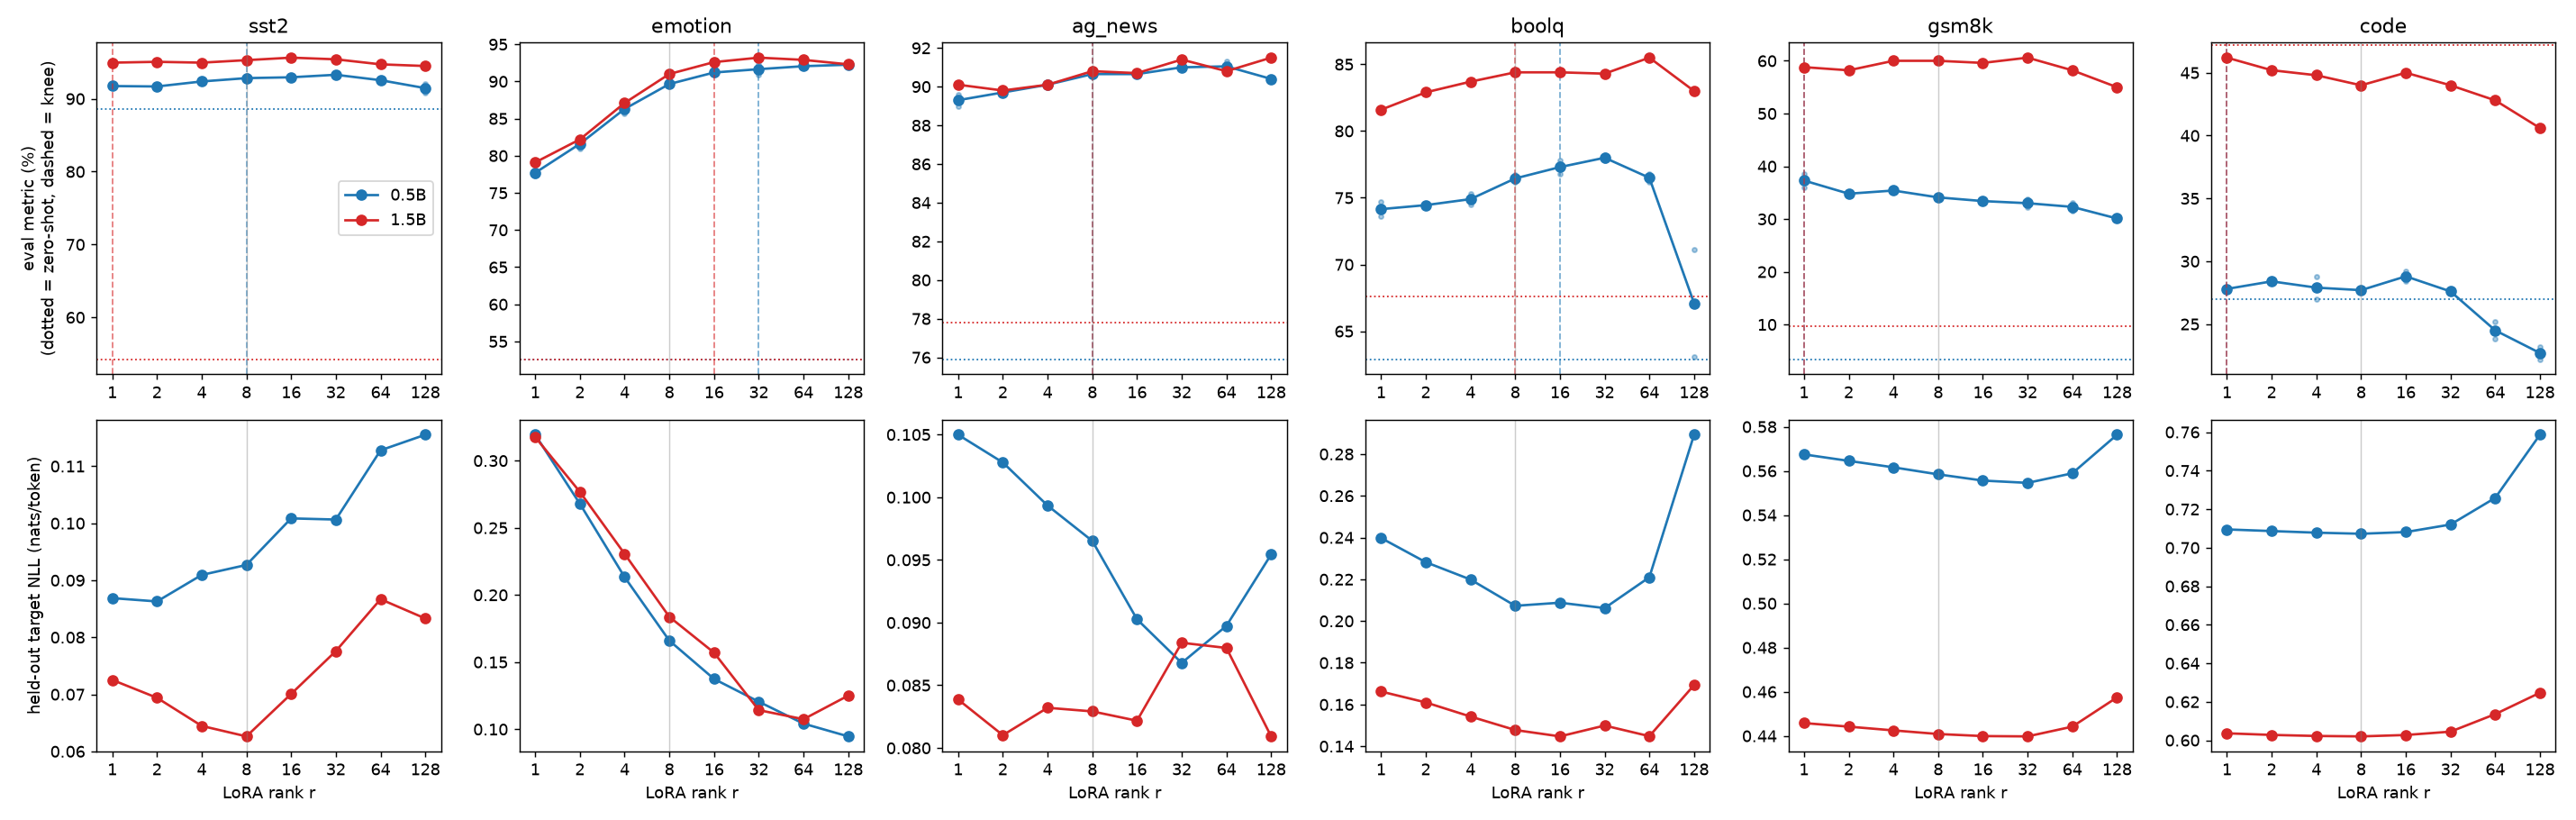
\includegraphics[width=\linewidth]{figures/rank_curves.png}
    \caption{Rank curves at learning rate $2\times10^{-4}$. \figtop\ Evaluation metric vs.\ \lora rank (lines are seed means, faint dots are individual seeds, dotted lines are zero-shot, dashed vertical lines are knees, grey line marks $r{=}8$). \figbottom\ Held-out target NLL. Only \emotion has a steep, monotone rank curve. \gsm and code decline with rank, and their NLL worsens at $r\geq64$. Curve shapes are nearly identical for 0.5B (blue) and 1.5B (red).}
    \label{fig:rank_curves}
\end{figure}

\Tabref{tab:rank_grid} and \figref{fig:rank_curves} show the main grid. {\bf Does the best rank vary across tasks?} Yes: it ranges from $r{=}1$ (0.5B \gsm, 1.5B code) to $r{=}128$ (0.5B \emotion, 1.5B \agnews). But the task ordering is not the one the folk wisdom predicts.

\para{Classification is flat.} On \sst and \agnews, $r{=}1$ is already within 1.3\pp of the best rank for 0.5B, and the curve barely moves after $r{=}8$.

\para{Emotion is the one steep curve.} 6-way \emotion rises from 77.7\% at $r{=}1$ to 89.7\% at $r{=}8$ and 92.3\% at $r{=}128$ on 0.5B. 1.5B follows the same shape.

\para{Math and code prefer low rank.} \gsm accuracy falls almost monotonically with rank on 0.5B: 37.3\% at $r{=}1$, 34.1\% at $r{=}8$, and 30.1\% at $r{=}128$. Held-out NLL stays nearly flat (0.555--0.568) up to $r{=}64$ and then worsens. On \code, fine-tuning barely beats zero-shot on 0.5B (best 28.8\% at $r{=}16$ vs.\ 27.0\%), and $r{=}128$ drops to 22.7\%, below zero-shot. On 1.5B, every code adapter scores below the 47.2\% zero-shot pass@1.

\para{Large ranks can collapse.} \boolq rises to 78.0\% at $r{=}32$ and then drops to 67.1\% at $r{=}128$ (seeds: 63.1\% and 71.1\%). Together with \gsm and code, large ranks at the default learning rate cost 7--11\pp on three of six tasks for 0.5B.

\subsection{How much does $r{=}8$ cost?}
\label{sec:res_gap}

\begin{table}[t]
    \centering
    \caption{Knee ranks and the cost of the $r{=}8$ default at learning rate $2\times10^{-4}$. Gap = best $-$ $r{=}8$ (pp), with a paired-bootstrap 95\% CI over evaluation items. ``Best $r{>}8$'' is the gain of the best rank above 8 over $r{=}8$. Cross-fitted gaps choose the best rank on one seed and score it on the other (0.5B only). $p_\text{Holm}$ is Holm-adjusted over tasks. Rows with $p_\text{Holm}<0.05$ are in {\bf bold}. Only \emotion gains significantly from a rank above 8. The \gsm and 1.5B code gaps favour $r{=}1$, \ie a rank \emph{smaller} than 8.}
    \label{tab:gap}
    \resizebox{\textwidth}{!}{%
    \begin{tabular}{@{}llcccccccc@{}}
        \toprule
        \textbf{Model} & \textbf{Task} & \textbf{Best $r$} & \textbf{Knee} & \textbf{NLL knee} & \textbf{Gap (pp)} & \textbf{95\% CI} & \textbf{Cross-fit} & \textbf{Best $r{>}8$ $-$ $r8$} & $p_\text{Holm}$ \\
        \midrule
        \multirow{6}{*}{0.5B}
        & \sst     & 32  & 8  & 1 & 0.5 & [$-$0.5, 1.4] & 0.5 & 0.5 & 1.0 \\
        & {\bf \emotion} & {\bf 128} & {\bf 32} & {\bf 1} & {\bf 2.6} & {\bf [1.2, 4.0]} & {\bf 1.8} & {\bf 2.6} & {\bf $<$0.001} \\
        & \agnews  & 64  & 8  & 1 & 0.4 & [$-$0.4, 1.1] & 0.3 & 0.4 & 1.0 \\
        & \boolq   & 32  & 16 & 2 & 1.6 & [$-$0.1, 3.1] & 0.9 & 1.6 & 0.454 \\
        & \gsm     & 1   & 1  & 1 & 3.2 & [0.7, 5.7]    & 3.2 & $-$0.7 & 0.132 \\
        & \code    & 16  & 1  & 2 & 1.1 & [$-$0.3, 2.5] & 0.7 & 1.1 & 0.89 \\
        \midrule
        \multirow{6}{*}{1.5B}
        & \sst     & 16  & 1  & 1 & 0.3 & [$-$0.5, 1.3] & -- & 0.3 & 1.0 \\
        & {\bf \emotion} & {\bf 32} & {\bf 16} & {\bf 1} & {\bf 2.2} & {\bf [0.8, 3.6]} & -- & {\bf 2.2} & {\bf 0.018} \\
        & \agnews  & 128 & 8  & 1 & 0.7 & [$-$0.5, 1.9] & -- & 0.7 & 1.0 \\
        & \boolq   & 64  & 8  & 1 & 1.1 & [$-$0.6, 2.8] & -- & 1.1 & 1.0 \\
        & \gsm     & 32  & 1  & 1 & 0.6 & [$-$2.6, 3.8] & -- & 0.6 & 1.0 \\
        & \code    & 1   & 1  & 1 & 2.2 & [0.2, 4.2]    & -- & 1.0 & 0.324 \\
        \bottomrule
    \end{tabular}}
\end{table}


\Tabref{tab:gap} tests the rank-8 gap. {\bf H1 (rank needs vary $\geq 8\times$)} holds numerically: knees range from 1 to 32. However, the direction is reversed. \gsm and code have the \emph{lowest} knees ($r{=}1$ for both models), and \emotion has the highest ($r{=}32$ for 0.5B, $r{=}16$ for 1.5B).

{\bf H2 ($r{=}8$ costs 3--8\pp on high-rank tasks)} is not supported. The largest gain from any rank above 8 is $+2.6$\pp on 0.5B \emotion (CI [1.2, 4.0], $p_\text{Holm}<0.001$). It shrinks to $+1.8$\pp when cross-fitted across seeds, which removes the winner's-curse bias. On 1.5B \emotion the gain is $+2.2$\pp ($p_\text{Holm}=0.018$). These are the only significant gaps after correction. No generative task gains more than 1\pp from a rank above 8. On 0.5B \gsm the best rank above 8 is 0.7\pp \emph{worse} than $r{=}8$. The two largest uncorrected gaps, 0.5B \gsm ($+3.2$\pp, CI [0.7, 5.7]) and 1.5B code ($+2.2$\pp, CI [0.2, 4.2]), both favour $r{=}1$. On these tasks, $r{=}8$ is too large, not too small.

\subsection{The rank effect is mostly a learning-rate effect}
\label{sec:res_lr}

\begin{table}[t]
    \centering
    \caption{Rank $\times$ learning-rate sweep on \qsmall (seed 0). Metric in \%. The best value in each (task, rank) column is in {\bf bold}. ``Best over lr'' takes the per-rank maximum. With a tuned learning rate, the spread across ranks is 0.7\pp on \emotion, 1.8\pp on \code, and 3.6\pp on \gsm (favouring $r{=}8$ over $r{=}128$).}
    \label{tab:lr}
    \small
    \begin{tabular}{@{}lcccc@{\hskip 14pt}cccc@{\hskip 14pt}cccc@{}}
        \toprule
        & \multicolumn{4}{c}{\textbf{\emotion}} & \multicolumn{4}{c}{\textbf{\gsm}} & \multicolumn{4}{c}{\textbf{\code}} \\
        \cmidrule(lr){2-5} \cmidrule(lr){6-9} \cmidrule(lr){10-13}
        \textbf{lr} & $r2$ & $r8$ & $r32$ & $r128$ & $r2$ & $r8$ & $r32$ & $r128$ & $r2$ & $r8$ & $r32$ & $r128$ \\
        \midrule
        $2\times10^{-5}$ & -- & -- & -- & -- & -- & 36.2 & -- & {\bf 34.0} & -- & 28.4 & -- & {\bf 27.8} \\
        $5\times10^{-5}$ & 68.9 & 77.5 & 87.0 & 92.1 & 35.8 & {\bf 37.6} & {\bf 35.0} & 30.2 & 28.6 & 28.4 & {\bf 29.6} & {\bf 27.8} \\
        $1\times10^{-4}$ & 74.7 & 84.8 & 91.0 & {\bf 92.4} & {\bf 36.0} & 35.6 & 33.0 & 33.0 & {\bf 29.0} & {\bf 28.8} & 28.6 & 25.2 \\
        $2\times10^{-4}$ & 82.2 & 89.6 & {\bf 92.4} & {\bf 92.4} & 35.2 & 34.0 & 32.2 & 30.0 & 28.4 & 27.8 & 27.6 & 22.2 \\
        $5\times10^{-4}$ & 90.3 & {\bf 92.8} & {\bf 92.4} & 90.5 & 35.0 & 32.2 & 31.2 & 22.4 & {\bf 29.0} & 26.6 & 22.8 & 15.4 \\
        $1\times10^{-3}$ & {\bf 92.1} & {\bf 92.8} & -- & -- & -- & -- & -- & -- & -- & -- & -- & -- \\
        $2\times10^{-3}$ & 91.7 & 91.0 & -- & -- & -- & -- & -- & -- & -- & -- & -- & -- \\
        \midrule
        Best over lr & 92.1 & 92.8 & 92.4 & 92.4 & 36.0 & 37.6 & 35.0 & 34.0 & 29.0 & 28.8 & 29.6 & 27.8 \\
        \bottomrule
    \end{tabular}
\end{table}


\begin{figure}[t]
    \centering
    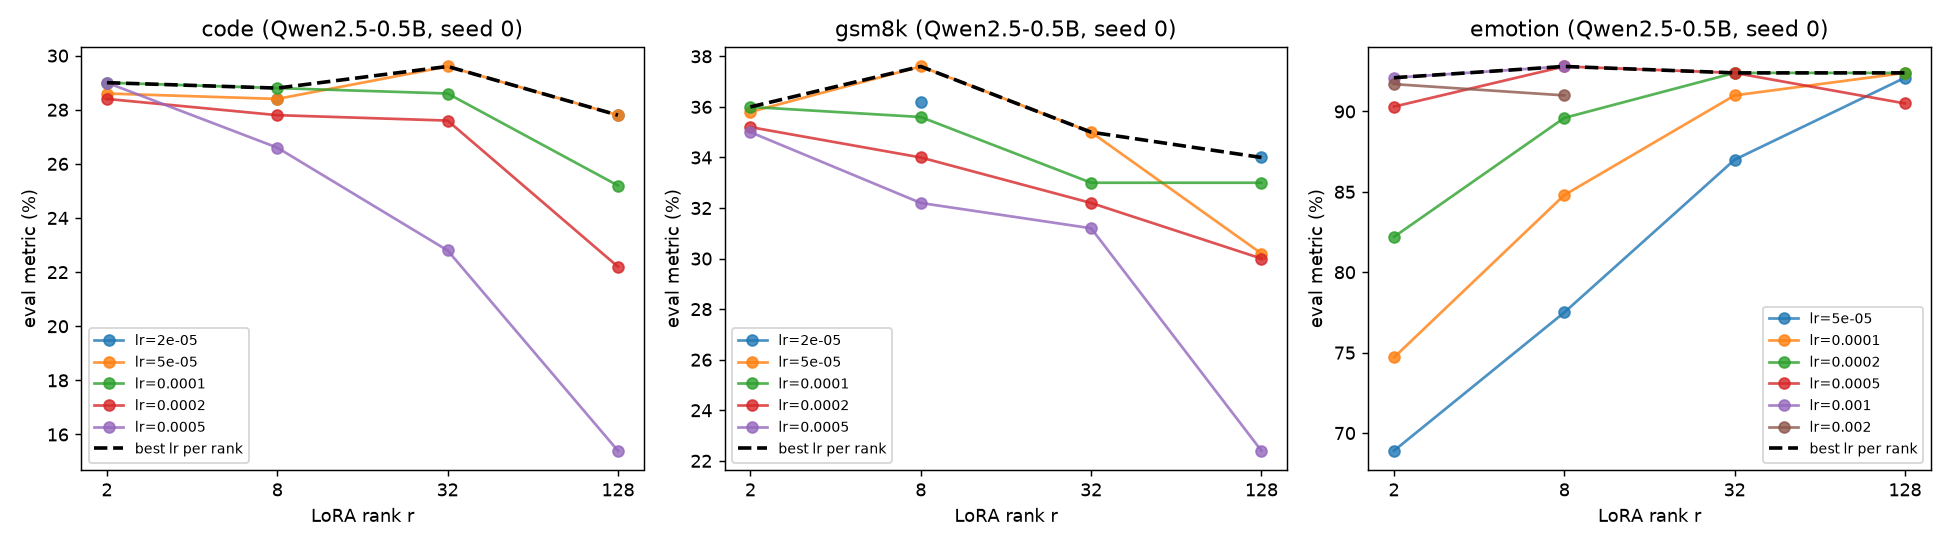
\includegraphics[width=\linewidth]{figures/lr_sweep.png}
    \caption{Metric vs.\ rank for each learning rate on \qsmall (seed 0). The dashed black line takes the best learning rate per rank. \figright\ On \emotion, low learning rates produce a steep ``needs high rank'' curve, while learning rates of $5\times10^{-4}$--$10^{-3}$ give a flat curve. \figleft\ and \figcenter\ On \code and \gsm, high rank never helps, and high rank combined with a high learning rate is destructive.}
    \label{fig:lr_sweep}
\end{figure}

\Tabref{tab:lr} and \figref{fig:lr_sweep} show the rank $\times$ learning-rate sweep. {\bf Does the \emotion gap survive learning-rate tuning?} No. At learning rate $5\times10^{-5}$, \emotion accuracy climbs from 68.9\% ($r{=}2$) to 92.1\% ($r{=}128$), a textbook ``needs high rank'' curve. At $5\times10^{-4}$--$10^{-3}$ the curve is flat: 92.1\% ($r{=}2$), 92.8\% ($r{=}8$), 92.4\% ($r{=}32$), 92.4\% ($r{=}128$). The best-over-lr spread across ranks is only 0.7\pp, and $r{=}8$ is the best rank. By contrast, the learning rate changes $r{=}8$ accuracy by 15.3\pp (77.5\% to 92.8\%). The explanation is the $\alpha=2r$ scaling: the update $2\mB\mA$ is a sum of $r$ rank-1 terms trained at the same learning rate, so a larger rank acts like a larger step. A low rank at a higher learning rate reaches the same accuracy.

On \gsm, the best-over-lr accuracy is highest at $r{=}8$ (37.6\%, learning rate $5\times10^{-5}$) and lowest at $r{=}128$ (34.0\%, $2\times10^{-5}$). High rank never helps, and at a high learning rate it is destructive ($r{=}128$ at $5\times10^{-4}$: 22.4\%). On \code, best-over-lr pass@1 is flat (27.8--29.6\%) and within noise (SE $\approx$ 2\pp). $r{=}128$ at $5\times10^{-4}$ falls to 15.4\%, with held-out NLL rising from 0.708 to 0.857.

The best learning rate shrinks as rank grows on all three tasks: on \emotion from $10^{-3}$ ($r{=}2$) to $10^{-4}$--$2\times10^{-4}$ ($r{=}128$), on \gsm from $10^{-4}$ to $2\times10^{-5}$, and on \code from $10^{-4}$/$5\times10^{-4}$ to $2\times10^{-5}$/$5\times10^{-5}$. This is the coupling expected under $\alpha\propto r$. The common recipe of ``$r{=}8$ with learning rate $2\times10^{-4}$'' is a matched pair. Changing the rank without changing the learning rate creates apparent rank effects.

\subsection{Does the knee shrink with model size?}
\label{sec:res_size}

\begin{table}[t]
    \centering
    \caption{Effect of model size at learning rate $2\times10^{-4}$. The knee is lower for 1.5B on 3 tasks, equal on 3, and never higher (sign test $p=0.25$). The clearest size effect is robustness to large ranks: on \boolq, $r{=}128$ costs 10.9\pp at 0.5B but 2.5\pp at 1.5B.}
    \label{tab:size}
    \small
    \begin{tabular}{@{}lcccccc@{}}
        \toprule
        & \multicolumn{2}{c}{\textbf{Knee}} & \multicolumn{2}{c}{\textbf{Best rank}} & \multicolumn{2}{c}{\textbf{$r128 -$ best (pp)}} \\
        \cmidrule(lr){2-3} \cmidrule(lr){4-5} \cmidrule(lr){6-7}
        \textbf{Task} & 0.5B & 1.5B & 0.5B & 1.5B & 0.5B & 1.5B \\
        \midrule
        \sst     & 8  & {\bf 1}  & 32  & 16  & $-$1.8  & $-$1.1 \\
        \emotion & 32 & {\bf 16} & 128 & 32  & 0.0     & $-$0.9 \\
        \agnews  & 8  & 8        & 64  & 128 & $-$0.7  & 0.0 \\
        \boolq   & 16 & {\bf 8}  & 32  & 64  & $-$10.9 & $-$2.5 \\
        \gsm     & 1  & 1        & 1   & 32  & $-$7.2  & $-$5.6 \\
        \code    & 1  & 1        & 16  & 1   & $-$6.1  & $-$5.6 \\
        \bottomrule
    \end{tabular}
\end{table}


\Tabref{tab:size} compares the two model sizes. {\bf H3} is directionally consistent but not statistically supported. The knee is lower for 1.5B on \sst, \emotion, and \boolq, equal on the other three tasks, and never higher. A sign test on the three non-tied pairs gives $p=0.25$. The best rank moves in both directions. The fixed-learning-rate curves have nearly the same shape at both sizes (\figref{fig:rank_curves}). The clearest size effect is robustness: 1.5B suffers much less from the $r{=}128$ collapse on \boolq ($-2.5$\pp vs.\ $-10.9$\pp).

\subsection{Does the initial gradient spectrum predict rank needs?}
\label{sec:res_pred}

\begin{table}[t]
    \centering
    \caption{Gradient spectrum statistics at initialization (median over target matrices). \rninety, $r_{99}$: directions needed for 90\% / 99\% of gradient energy. \erank: entropy effective rank. Top-8: fraction of energy in the top 8 directions. The ordering code $\gg$ \gsm $>$ \boolq $>$ \agnews $>$ \emotion $>$ \sst is consistent across sizes.}
    \label{tab:gradid}
    \small
    \begin{tabular}{@{}lccccccc@{}}
        \toprule
        & \multicolumn{4}{c}{\textbf{\qsmall}} & \multicolumn{3}{c}{\textbf{\qlarge}} \\
        \cmidrule(lr){2-5} \cmidrule(lr){6-8}
        \textbf{Task} & \rninety & $r_{99}$ & \erank & Top-8 & \rninety & $r_{99}$ & \erank \\
        \midrule
        \sst     & 2 & 4   & 7.4   & 0.999 & 2 & 5   & 10.2 \\
        \emotion & 2 & 5   & 10.3  & 0.999 & 2 & 5   & 12.3 \\
        \agnews  & 2 & 5   & 17.0  & 0.997 & 2 & 5   & 18.6 \\
        \boolq   & 2 & 7   & 26.1  & 0.993 & 2 & 6.5 & 22.4 \\
        \gsm     & 4 & 9   & 46.3  & 0.990 & 4 & 11  & 80.4 \\
        \code    & 6 & 143 & 223.7 & 0.919 & 3 & 89  & 244.2 \\
        \bottomrule
    \end{tabular}
\end{table}


\begin{figure}[t]
    \centering
    \begin{subfigure}[b]{0.8\textwidth}
        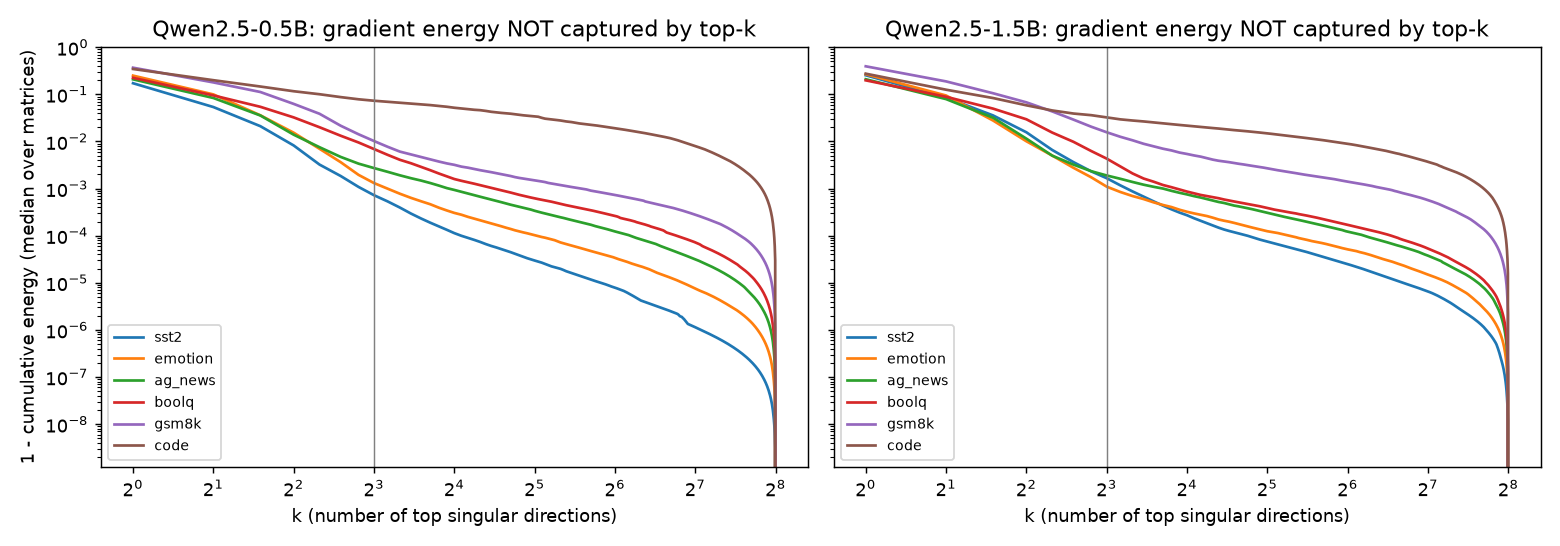
\includegraphics[width=\textwidth]{figures/gradient_spectra.png}
        \caption{Gradient energy outside the top-$k$ directions}
        \label{fig:spectra}
    \end{subfigure}
    \\[4pt]
    \begin{subfigure}[b]{0.95\textwidth}
        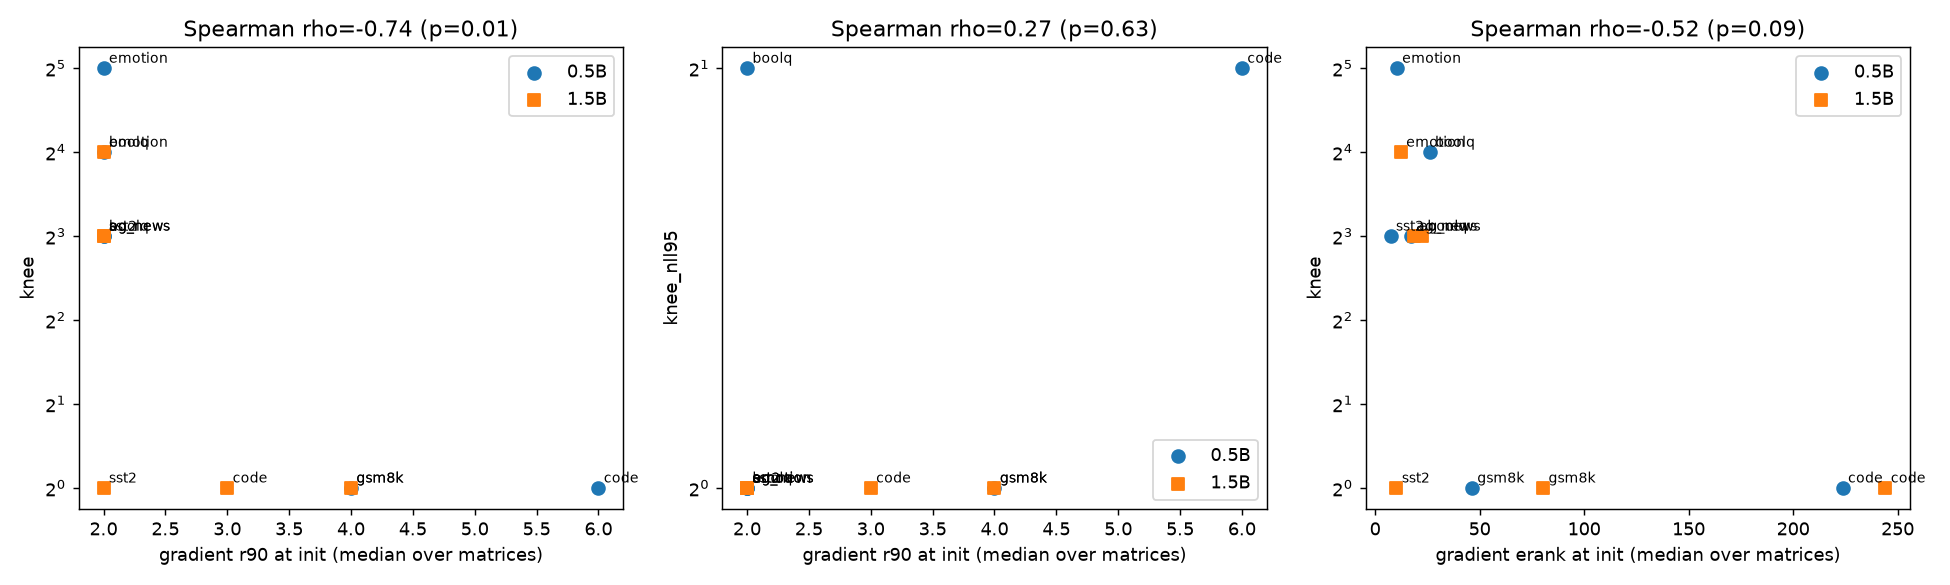
\includegraphics[width=\textwidth]{figures/gradid_vs_knee.png}
        \caption{Gradient statistic vs.\ empirical knee}
        \label{fig:gradid_knee}
    \end{subfigure}
    \caption{The gradient-spectrum predictor. \captiona\ Fraction of gradient energy not captured by the top-$k$ singular directions, median over target matrices, for 0.5B (left) and 1.5B (right). Spectra are truncated at 256, so curves drop to 0 there by construction. The grey line marks $k{=}8$. Code has by far the heaviest tail. \captionb\ \rninety (left), \rninety vs.\ NLL knee (middle), and \erank (right) against the knee rank (log scale). Tasks with the heaviest gradient tails (code, \gsm) have the \emph{lowest} knees.}
    \label{fig:gradid}
\end{figure}

\Tabref{tab:gradid} and \figref{fig:spectra} show that the gradient statistic separates tasks cleanly and consistently across model sizes. The code gradient spreads over two orders of magnitude more directions than \sst (\erank 223.7 vs.\ 7.4 on 0.5B), and only 91.9\% of its energy lies in the top 8 directions, compared with 99.9\% for \sst.

{\bf H4 (the statistic predicts the knee with $\rho>0.7$)} is refuted, with a significant correlation of the opposite sign (\tabref{tab:predictor}, \figref{fig:gradid_knee}). The primary predictor \rninety has $\rho=-0.74$ ($p=0.014$) with the knee. All other gradient statistics also correlate negatively ($\rho$ from $-0.52$ to $-0.63$). With a leave-one-out calibrated scale, \rninety lands within $2\times$ of the knee for 0 of 12 pairs, while always predicting $r{=}8$ succeeds for 6 of 12. The NLL knee shows a weak positive correlation ($\rho=0.27$, $p=0.63$). Its high hit rate (0.92) is not informative, because NLL knees are 1 or 2 for every pair.

\begin{table}[t]
    \centering
    \caption{How well initial-gradient statistics predict rank needs over $n=12$ (task, model) pairs. Positive $\rho$ means ``predicts higher rank'' (top-8 energy and zero-shot accuracy are sign-flipped). ``Within 2$\times$'' is the leave-one-out hit rate after fitting one multiplicative scale. All significant correlations with the knee are \emph{negative}, and no gradient statistic beats always predicting $r{=}8$ (best value per target in {\bf bold}).}
    \label{tab:predictor}
    \small
    \begin{tabular}{@{}llccc@{}}
        \toprule
        \textbf{Target} & \textbf{Predictor} & \textbf{Spearman $\rho$} & \textbf{Perm.\ $p$} & \textbf{Within 2$\times$} \\
        \midrule
        \multirow{7}{*}{Knee}
        & \rninety (primary) & $-$0.74 & 0.014 & 0.00 \\
        & $r_{99}$           & $-$0.58 & 0.059 & 0.00 \\
        & \erank             & $-$0.52 & 0.093 & 0.08 \\
        & Top-8 energy       & $-$0.63 & 0.029 & -- \\
        & Stable rank        & $-$0.57 & 0.061 & 0.00 \\
        & Zero-shot accuracy & $-$0.50 & 0.111 & -- \\
        & Constant $r{=}8$   & -- & -- & {\bf 0.50} \\
        \midrule
        \multirow{3}{*}{Best rank}
        & \rninety           & $-$0.64 & 0.029 & {\bf 0.42} \\
        & \erank             & $-$0.45 & 0.143 & 0.08 \\
        & Constant $r{=}8$   & -- & -- & 0.17 \\
        \midrule
        \multirow{2}{*}{NLL knee}
        & \rninety           & 0.27 & 0.632 & {\bf 0.92} \\
        & $r_{99}$           & 0.47 & 0.161 & 0.67 \\
        \bottomrule
    \end{tabular}
\end{table}


\section{Discussion}
\label{sec:discussion}

\begin{table}[t]
    \centering
    \caption{Verdicts on the pre-registered hypotheses.}
    \label{tab:verdicts}
    \small
    \begin{tabular}{@{}lp{3.6cm}p{8.2cm}@{}}
        \toprule
        \textbf{ID} & \textbf{Verdict} & \textbf{Evidence} \\
        \midrule
        H1 & Refuted in substance & Knees span 1--32 at a fixed learning rate, but code and \gsm are lowest and \emotion is highest. Best-over-lr curves are flat or favour low rank. \\
        H2 & Not supported & The maximum gain above $r{=}8$ is 2.6\pp (cross-fitted 1.8\pp), only on \emotion, and it vanishes with a tuned learning rate. \\
        H3 & Weak / inconclusive & The knee is lower for 1.5B on 3/6 tasks and never higher (sign test $p=0.25$). Best ranks move both ways. \\
        H4 & Refuted (opposite sign) & $\rho(\text{\rninety}, \text{knee}) = -0.74$, $p=0.014$. Factor-2 hit rate 0/12 vs.\ 6/12 for constant $r{=}8$. \\
        \bottomrule
    \end{tabular}
\end{table}

\Tabref{tab:verdicts} summarizes our verdicts. We now discuss why the results run against the common intuition.

\para{Why do math and code not need high rank here?}
We see three explanations that fit the data. First, {\bf SFT on 4,000 examples mostly teaches format, not capability}. Qwen2.5 base models saw a lot of math and code in pre-training~\citep{qwen2024qwen25}. Zero-shot \gsm accuracy is 3.4\% mainly because the base model does not emit the expected final-answer format, and $r{=}1$ already reaches 37.3\%. \mbpp gains are at most 2\pp. Learning a response format is a low-rank change. The high-rank regime of \citet{biderman2024lora} involves billions of tokens of continued pre-training, which is a different setting. Second, {\bf a higher rank means a larger effective step and more forgetting}. Under $\alpha=2r$, large ranks at a fixed learning rate overfit the small SFT set and damage pretrained skills. Held-out NLL worsens at $r\geq 64$ on \gsm and code, and every collapse we observe coincides with worse NLL. Third, {\bf \emotion is the exception because its labels are idiosyncratic}. Distinctions such as ``love'' vs.\ ``joy'' are noisy and dataset-specific, and the base model does not already encode them (52.6\% zero-shot). \emotion therefore needs the most movement away from the base model, and at a fixed learning rate only more rank delivers that movement.

\para{Why does the gradient predictor fail?}
At initialization, the mean gradient is dominated by one or two directions in every task: the median stable rank is 1.2--1.7, and $r_{50}=1$. The tail that \rninety and \erank measure reflects how diverse the token-level targets are. Code has the most varied output tokens, and \sst has a single label token. Diverse targets do not mean that the \emph{solution} needs many directions: the best code and \gsm adapters have rank 1--16. The predictor also ignores the rank--learning-rate coupling, which dominates the empirical knees. A useful predictor probably needs information from training, such as the spectrum of $\Delta\mW$ after a short pilot run.

\para{Failure modes.}
The high-rank collapses (\boolq $r{=}128$, code $r{=}128$, \gsm $r{=}128$ at learning rate $5\times10^{-4}$) all come with worse held-out NLL. They reflect overfitting or instability, not a lack of capacity. On 1.5B code, every adapter is below the zero-shot \mbpp score, because the alpaca-style training instructions do not match \mbpp's prompt and assert format. The 1.5B code knee therefore mostly measures how little damage each rank does.

\para{Limitations.}
Our models are small (0.5B and 1.5B) and come from one family. The 1.5B grid has one seed, so H3 rests on two sizes and is underpowered. The results may not transfer to 7B+ models or other families. We use 4,000 examples and one epoch per task. Rank needs may grow with much larger SFT sets or with continued pre-training. We study one parameterization ($\alpha=2r$ on all linear layers). rsLoRA scaling~\citep{kalajdzievski2023rslora} or attention-only targets would change the rank--learning-rate coupling. The learning-rate sweep covers only 3 tasks, 4 ranks, one model, and one seed. Evaluation sets of 500--1,000 items give standard errors of 1--2\pp, which is comparable to many differences between neighbouring ranks. We therefore base our conclusions on monotone trends and learning-rate interactions rather than on single-rank comparisons. The gradient predictor used 128 examples and one seed, and we did not test alternatives such as per-example gradient covariance. Finally, we used Hugging Face generation with greedy decoding, and timings are not comparable across runs because the GPUs were shared.

\para{Broader implications.}
For practitioners, our results suggest a simple rule: sweeping the learning rate is worth much more than sweeping the rank. Keeping $r\approx 8$--16 also saves memory and compute compared with large ranks. A negative result like ours can also prevent wasted effort on rank searches. We see no direct negative societal impact from this study beyond the general risks of fine-tuning language models.

\section{Conclusion}
\label{sec:conclusion}

We asked whether the default \lora rank of 8 is a blind spot for tasks such as math and code. In a controlled sweep of about 200 adapters on \qsmall and \qlarge, the best rank was not a stable property of the task. At a fixed learning rate it ranged from 1 to 128, but the ordering contradicted the intuition: \gsm and code preferred low rank, and only 6-way \emotion classification gained significantly from more rank ($+2.6$\pp). Once we tuned the learning rate per rank, that gain disappeared, and $r{=}8$ was the best rank or within 0.8\pp of it on all three tasks in our learning-rate sweep. The spectrum of the initial gradient ordered tasks consistently but anti-predicted the needed rank ($\rho=-0.74$, $p=0.014$).

{\bf The key takeaway is that, in small-data SFT, the default rank is not the blind spot; the default learning rate at a non-default rank is.} We recommend keeping $r\approx 8$--16, lowering the learning rate as rank grows (roughly $\propto 1/\sqrt{r}$ to $1/r$ under $\alpha=2r$), and avoiding $r\geq 64$ with standard scaling on small SFT sets.

Future work should (1) repeat the study at 7B+ scale and with $\geq$100k-example or continued pre-training data, where high-rank benefits have been reported; (2) run the full rank $\times$ learning-rate grid with rsLoRA scaling; (3) test predictors based on a short pilot run, such as the spectrum of $\Delta\mW$ after 20 steps; and (4) use more seeds and larger evaluation sets for the generative tasks.


\bibliography{references}

\end{document}
